\documentclass[11pt]{beamer}

%%%%%%%%%%%%%%%%%%%%%
\usepackage[italian]{babel}
%\usepackage[latin1]{inputenc}
%\usepackage{times}
\usepackage{pgf}
\usepackage{xcolor}
\usepackage{multimedia}
\usepackage{ragged2e}
\usepackage{textcomp}
\usepackage[nice]{nicefrac}
%\usepackage[adobe-utopia]{mathdesign}
%\usepackage{amsmath, amsfonts, amssymb, amsthm, mathrsfs}
\usepackage[OMLmathrm, OMLmathbf, sfdefault=cmbr]{isomath}
%%%
\newcommand{\quotes}[1]{{``#1''}}
\newcommand{\acgrave}[1]{\`{#1}}
\newcommand{\itt}[1]{\textit{#1}}
\newcommand{\mrm}[1]{\mathrm{#1}}
\newcommand{\itm}[1]{\mathit{#1}}
\newcommand{\mbf}[1]{\mathbf{#1}}
\newcommand{\mat}[1]{\mathbf{#1}}
\newcommand{\vect}[1]{\lowercase{ \mathbf{#1}}}
\newcommand{\dyad}[1]{\overline{\overline{#1}}}
\newcommand{\mbfit}[1]{\mathbold{#1}}
\newcommand{\�}[0]{\textrm{\textdegree}}
\newcommand{\spanning}[1]{ \mathrm{span} \left \{ #1 \right \} }
\newcommand{\colspan}[1]{ \mathrm{colspan} \left \{ #1 \right \} }
\newcommand{\kernel}[1]{ \mathrm{ker} \left \{ #1 \right \} }
\newcommand{\rank}[1]{ \mathrm{rank} \left ( #1 \right ) }
%\newcommand{\myalert}[1]{\color{mycolor}\textbf{#1} \color{black}}

\newcommand{\putlink}[1]{%
 \pgfsetlinewidth{1.4pt}%
 \pgfsetendarrow{\pgfarrowtriangle{4pt}}%
 \pgfline{\pgfxy(1,1)}{\pgfxy(#1,1)}
}
%%%
%\usepackage[]{hyperref}%[colorlinks]
\hypersetup{ 
	pdfstartview={FitV}, % {FitH FitV XYZ null null 1}
	pdfpagelayout=SinglePage, % SinglePage OneColumn TwoColumnRight
	pdfdirection=L2R,
	pdfpagemode = {UseNone}, % UseNone, UseThumbs, UseOutlines, FullScreen, UseOC, UseAttachments
	pdfsubject = {Model Order Reduction in Finite Element Analysis of Phased Arrays},
	pdfkeywords = {Model Order Reduction, Finite Element Method, Near to Far Fields Transformations, Phased Arrays},
	pdfauthor = {Laurent Ntibarikure},
	pdfproducer = {Laurent Ntibarikure},
	pdfcenterwindow = true,
	pdfdisplaydoctitle = true,
	bookmarksopen=true,
	bookmarksnumbered,
	bookmarksopenlevel=\maxdimen, % -1,  \maxdimen 
	CJKbookmarks=true,
	bookmarkstype=toc,
	pdffitwindow=false,
}
\mode<presentation>
{
\usetheme{Malmoe}
\setbeamercovered{transparent}
  % or whatever (possibly just delete it)
\definecolor{mywhite}{rgb}{1,1,1}
\definecolor{mycolor}{rgb}{.122,.286,.490}
\definecolor{miorosso}{RGB}{139,35,35}
\definecolor{miogrigio}{RGB}{229,229,229}
\setbeamercolor{item}{fg=mycolor}
\setbeamercolor{title}{fg=mycolor}
\setbeamercolor{frametitle}{fg=mycolor}
\setbeamercolor{frametitle}{bg=miogrigio}
\setbeamercolor{alerted text}{fg=mycolor}
\setbeamercolor{subsection in head/foot}{bg=mycolor}
\setbeamercolor{section in head/foot}{bg=black}
\setbeamercolor{section in toc}{fg=mycolor}
\setbeamercolor{title in head/foot}{bg=mycolor}

%\setbeamerfont{subsection in head/foot}{size=\footnotesize}
%\setbeamerfont{section in head/foot}{size=\footnotesize}
%\setbeamerfont{title in head/foot}{size=\footnotesize}
%\setbeamerfont{author in head/foot}{size=\footnotesize}
\setbeamerfont{frametitle}{size=\normalsize}
\setbeamerfont{framesubtitle}{size=\small,shape=\itshape}
\newenvironment{colorblock}[2]
{\setbeamercolor{item}{fg=#1,bg=#1}
\begin{beamerboxesrounded}[upper=#2,lower=#2,shadow=true]}
{\end{beamerboxesrounded}}
}

\graphicspath{{img/}}


\title[MOR for Phased Array Antennas]{\textsf{\Large{Model Order Reduction in Full-Wave \\ Analysis of Phased Array Antennas}}}
\author[Laurent Ntibarikure]{} %\thanks{Ciao}
\date[\today]{}
\institute[UniFi CEM -  UniSaarland LTE]{}
\logo{
\includegraphics[width=12.62cm]{logoUnifiSfondo.pdf}}
\subject{Model Order Reduction in Finite Element Analysis of Large Phased Array Antennas}


\begin{document}
%%%%% PRIMA PAGINA
\frame{
\begin{center}
\vspace{-0.1cm}\textsl{\scriptsize{Universit\`{a} degli Studi di Firenze - Facolt\`{a} di Ingegneria}}\\[0.5cm]%\\[-0.1cm]Departimento di Elettronica e Telecomunicazioni}}\\[0.5cm]
\normalsize{Tesi di Laurea Specialistica in \\ Ingegneria Elettronica}
\end{center}
\vspace{-.1cm}\maketitle 
\begin{center}
\vspace{-2.5cm} Laurent Ntibarikure \\[-3cm]
\end{center}
\vspace{-1cm}
\begin{table}[h]
\begin{tabular*}{\textwidth}[b]{rlll}
%\hspace{-.5cm} 

\includegraphics[width=1cm]{unifiLogo.pdf} \hspace{0.2cm} & & & %\hspace{-0.6cm} 

\includegraphics[width=1cm]{eule.pdf} \\[-.5cm]
& \hspace{-0.2cm} \scriptsize{Relatori:} & \hspace{-0.1cm}  \scriptsize{Relatori esterni:} & \\[.15cm]
& \scriptsize{Prof. Giuseppe Pelosi} & \hspace{0cm} \scriptsize{Prof. Romanus Dyczij-Edlinger} &\\
& \scriptsize{Dr. Ing. Stefano Selleri} & \hspace{0cm} \scriptsize{Dr. Ing. Ortwin Farle} &
\end{tabular*}
\end{table}
\begin{center}
\vspace{-.5cm}
\footnotesize{Anno Accademico 2008-2009}
\end{center}
}

%%%%% SUMMARY
%\section*{Sommario}
%\frame{\tableofcontents}

%%%% MOTIVAZIONI

\section{Motivazioni}
\subsection{Analisi numerica di array fasati di grandi dimensioni}
%% appl radar
\frame
{
\frametitle{Array fasati:\textnormal{ }\itt{pattern} di radiazione in eccitazione equifase}
\vspace{-.2cm}
%\begin{figure}
%\centering
%\begin{minipage}[l]{5cm}
%\hspace{-.5cm}
\centering
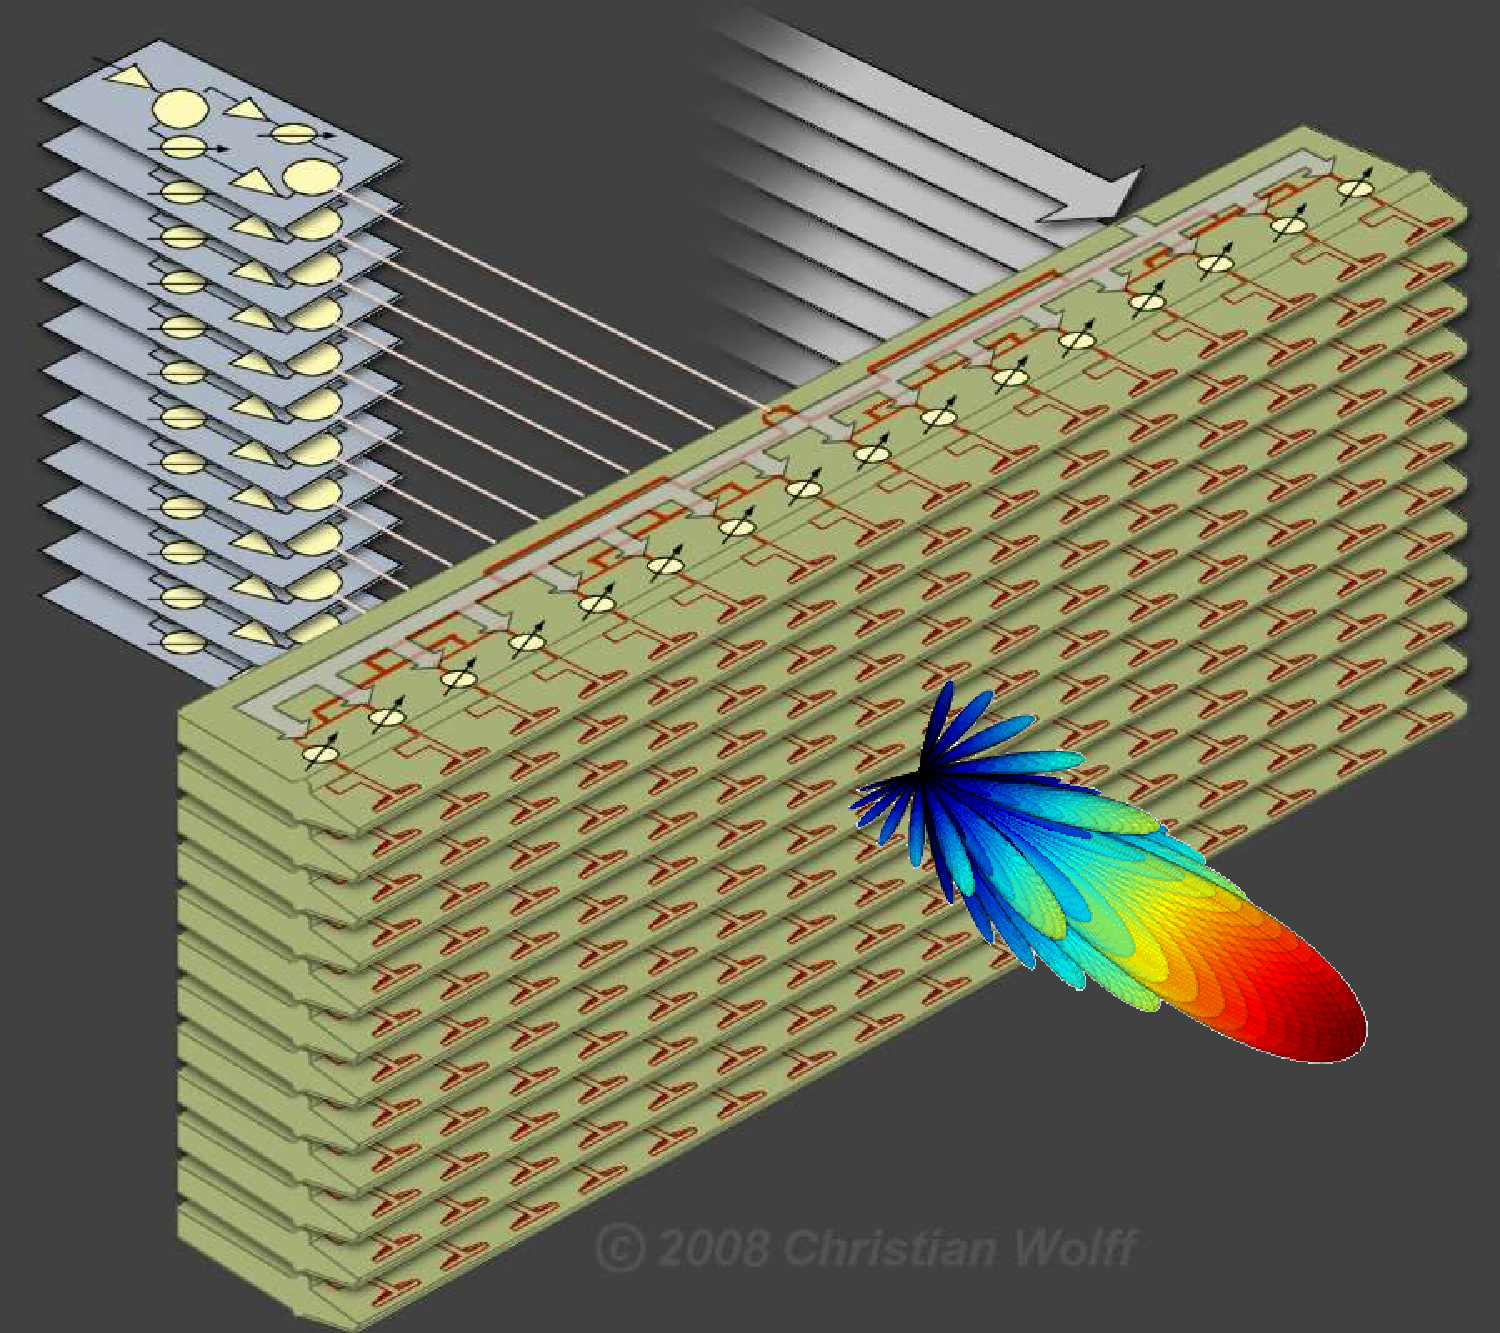
\includegraphics[width=6cm]{phasedArray1} \\
\tiny Array planare di 12 x 16 dipoli ripiegati su supporto dielettrico 
%\end{minipage}
%\hspace{1cm}

%\end{figure}	
}
\frame
{
\frametitle{Array fasati:  scansione nel piano azimutale}
\vspace{-.2cm}

\centering
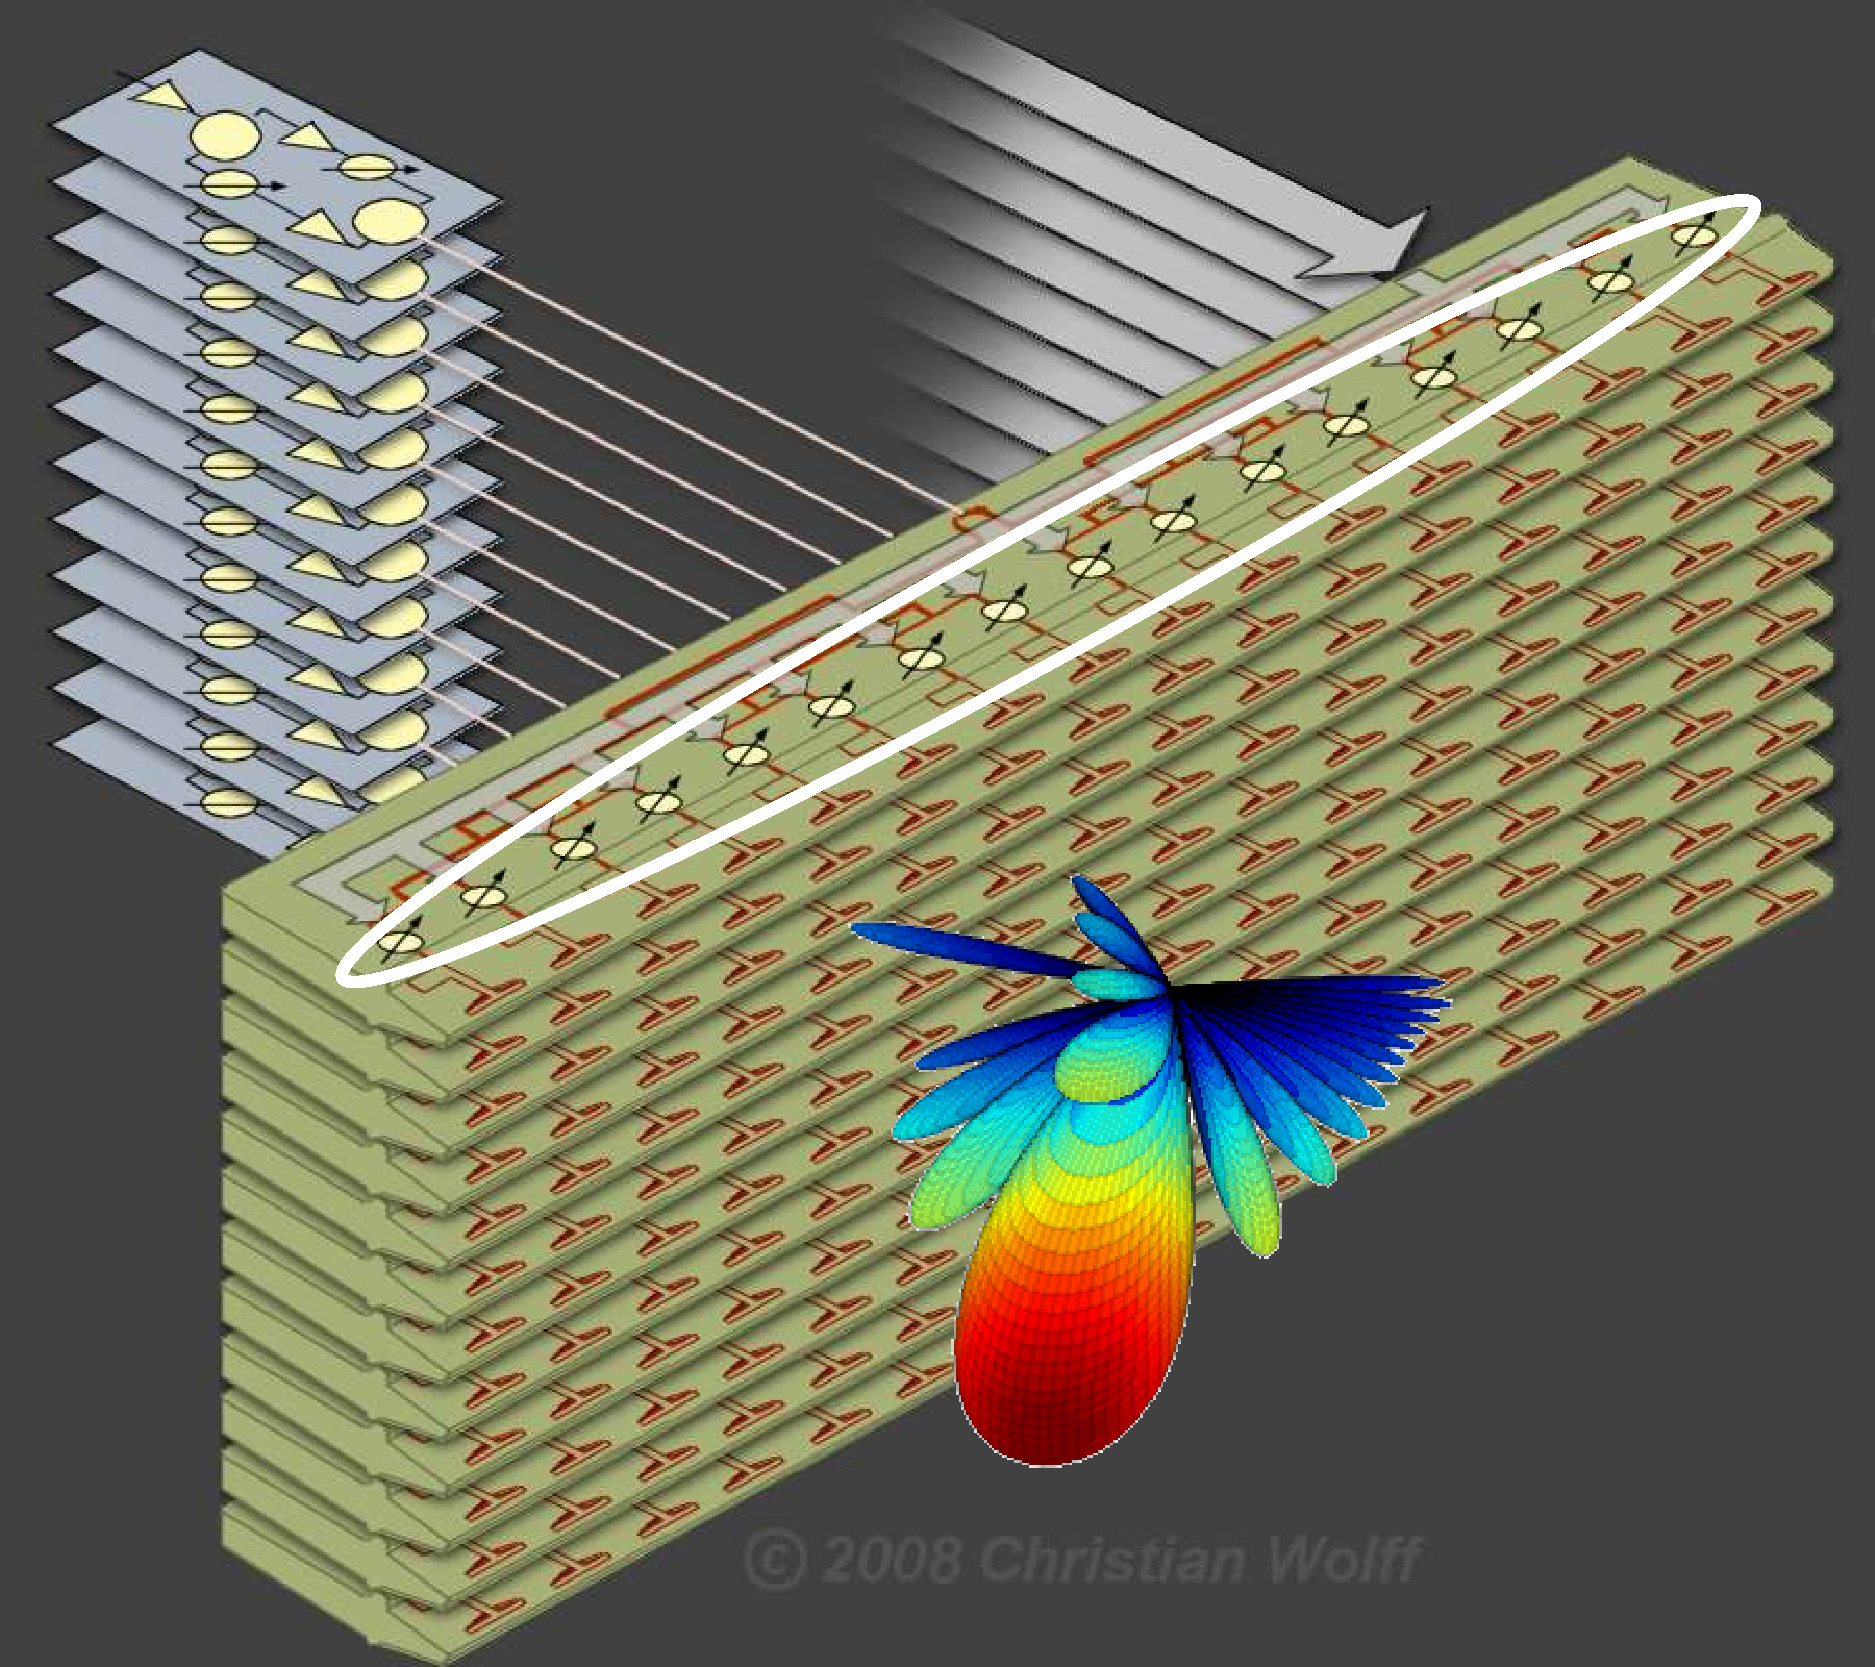
\includegraphics[width=6cm]{phasedArray2} \\
\tiny Array planare di 12 x 16 dipoli ripiegati su supporto dielettrico 

}
\frame
{
\frametitle{Array fasati: scansione nel piano di elevazione}
\vspace{-.2cm}

\centering
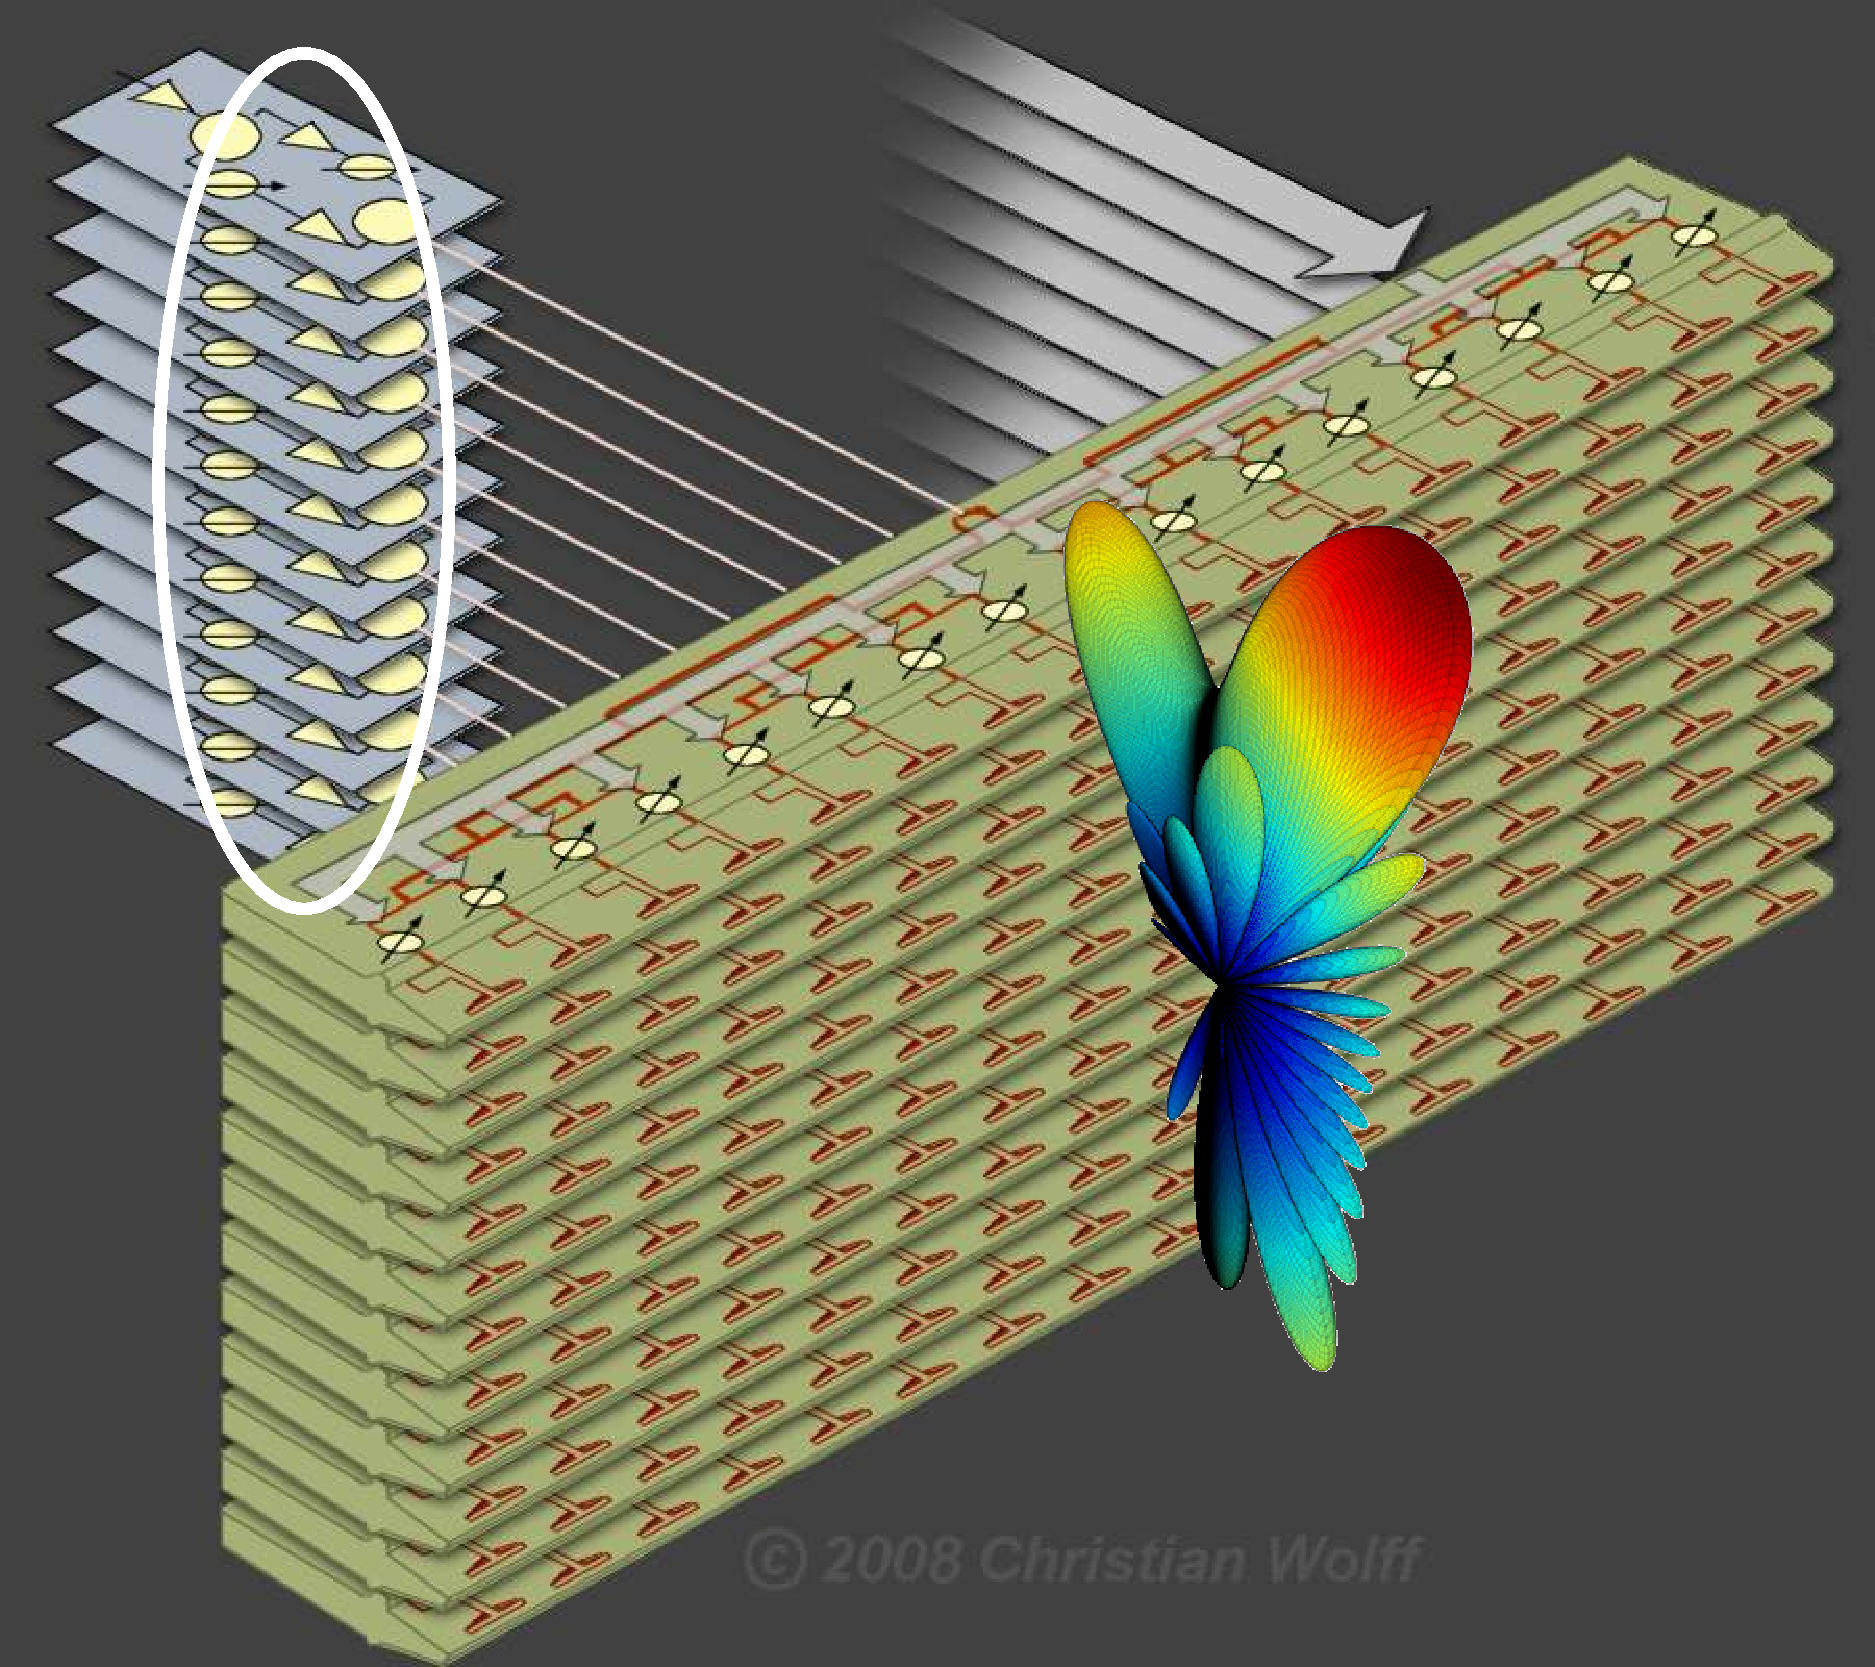
\includegraphics[width=6cm]{phasedArray3} \\
\tiny Array planare di 12 x 16 dipoli ripiegati su supporto dielettrico 

}
\frame
{
\frametitle{Array fasati: scansione nel semispazio individuato dal piano dell'array}
\vspace{-.2cm}

\centering
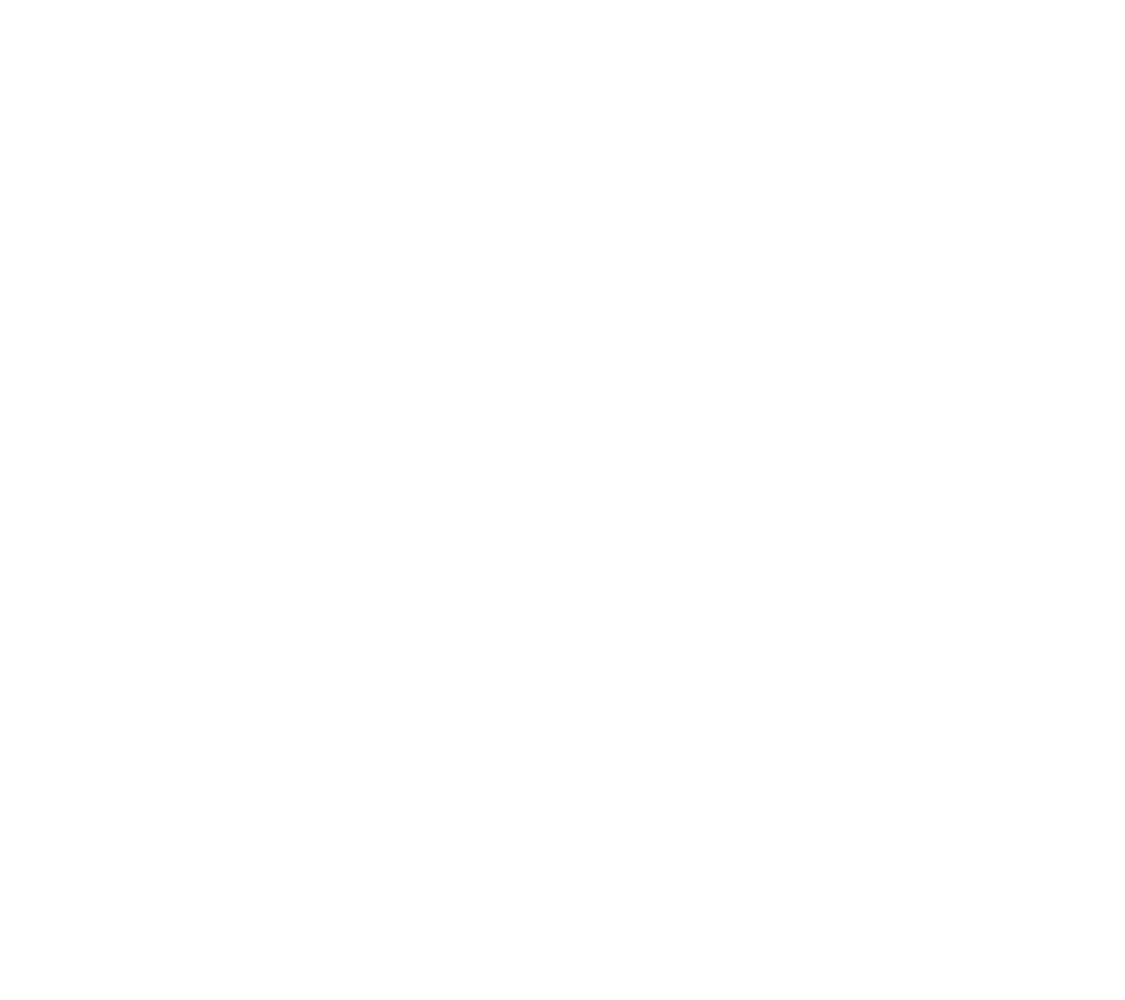
\includegraphics[width=6cm]{phasedArray4} \\
\tiny Array planare di 12 x 16 dipoli ripiegati su supporto dielettrico 

}
%% appl telecom
\frame
{
  \frametitle{Array fasati per applicazioni radaristiche e per le telecomunicazioni}
\vspace{-.2cm}
\begin{figure}
\centering
\begin{minipage}[l]{4cm}
\begin{minipage}[t]{4cm}
\centering
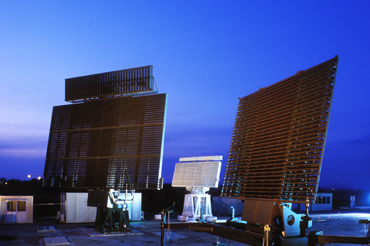
\includegraphics[width=4cm]{Rat31} \\
\tiny RAT 31 DL - SELEX Sistemi Integrati. D-band solid state phased array, 3D surveillance radar
\end{minipage}
\begin{minipage}[b]{4cm}
\centering
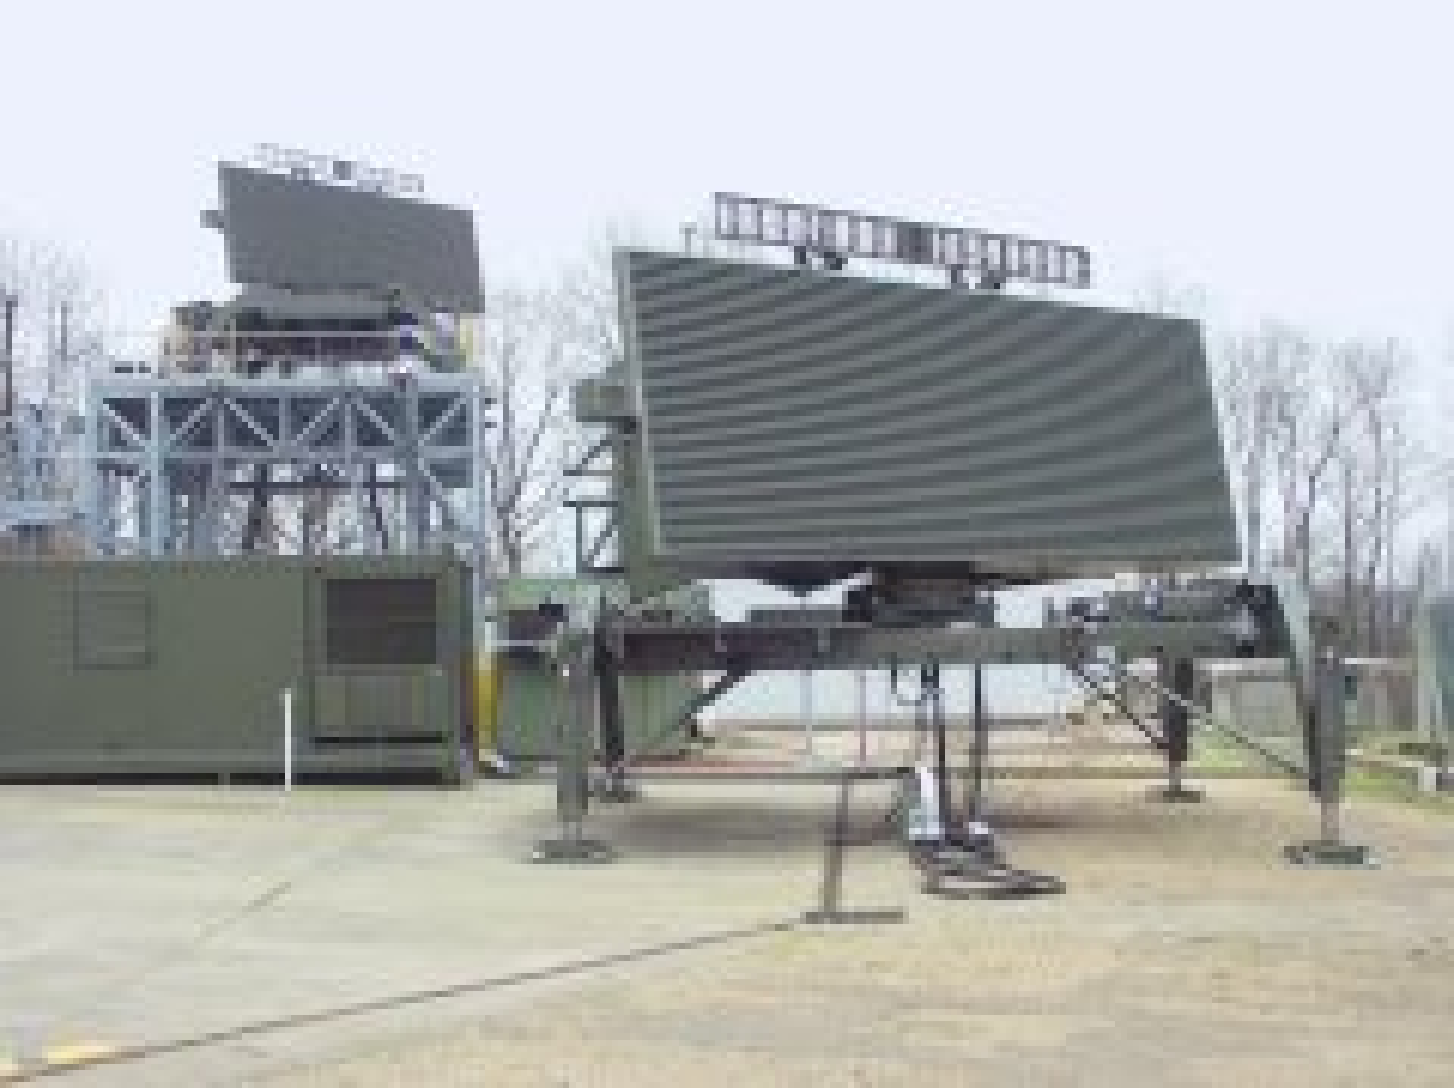
\includegraphics[width=4cm]{ThomsonMasterA} \\
\tiny Thomson Master-T Radar - \textcopyright Thomson CSF Air Command and Control Systems
\end{minipage}
\end{minipage}
\hspace{.8cm}
%\begin{minipage}[l]{5cm}
%\begin{minipage}[t]{5cm}
%\centering
%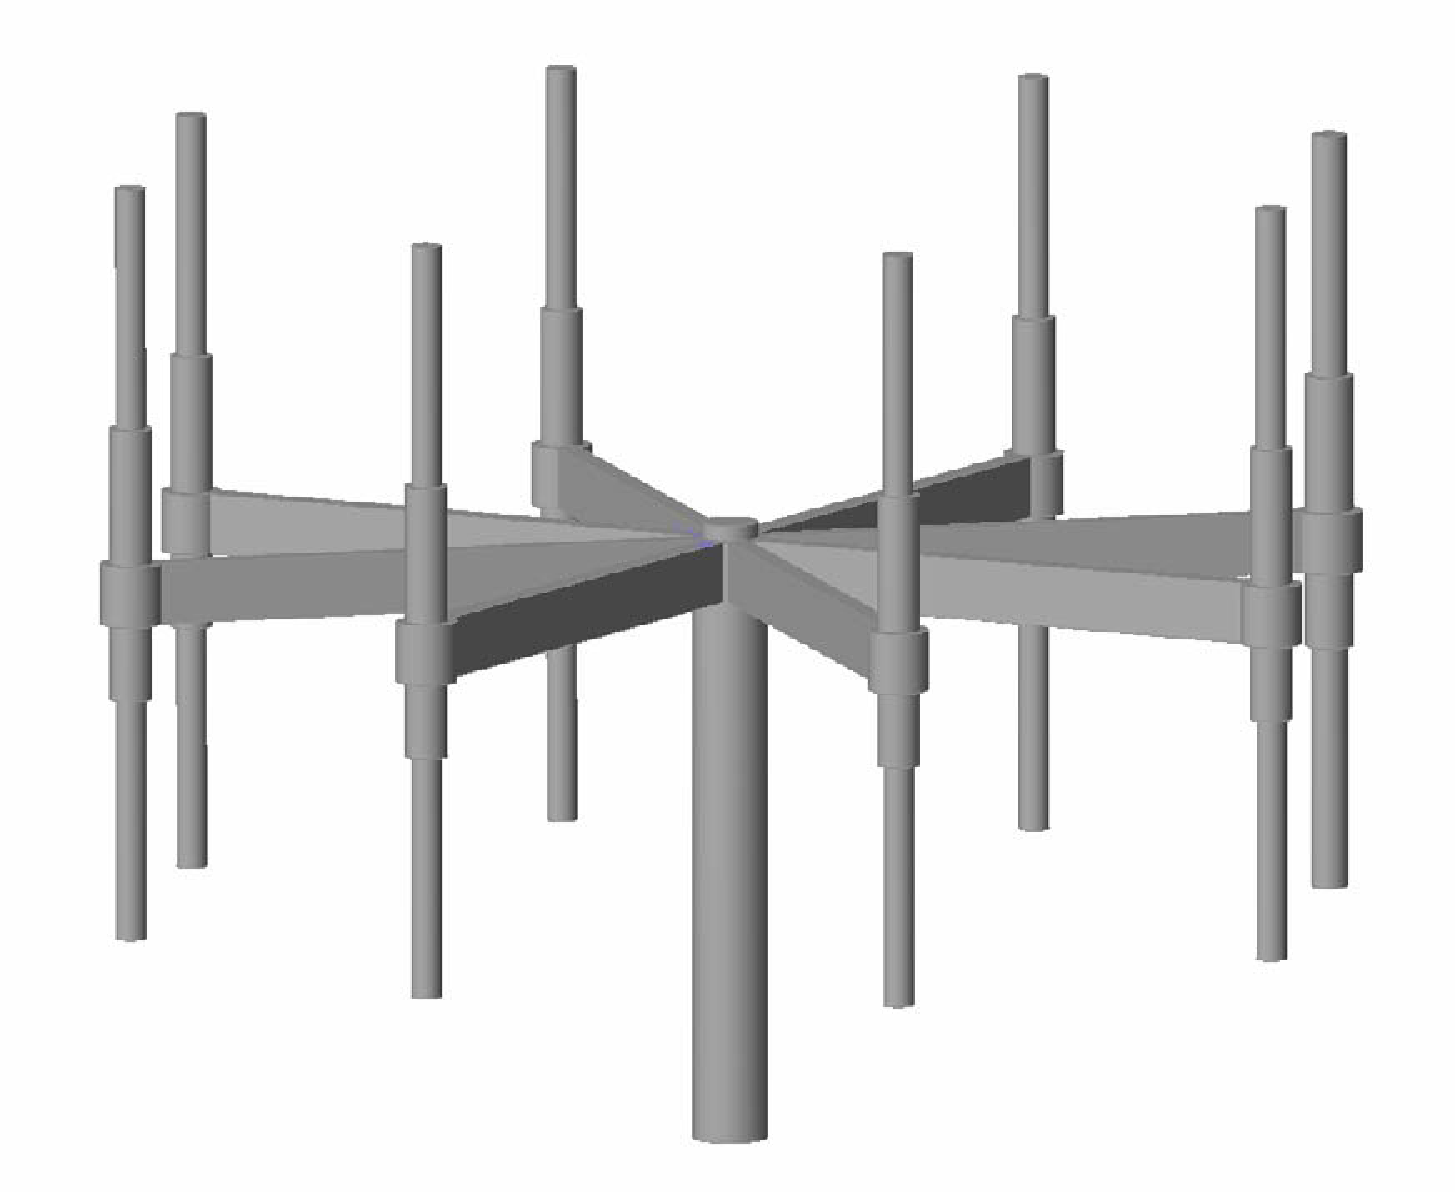
\includegraphics[width=3cm]{arrayDipSmart} \\
%\tiny W. Mahler, F.M. Landstorfer, \quotes{Design and Optimisation of an Antenna Array for WIMAX Base Stations}, University of Stuttgart, Institute of Radio Frequency Technology
%\end{minipage}
%\begin{minipage}[b]{5cm}
%\centering
%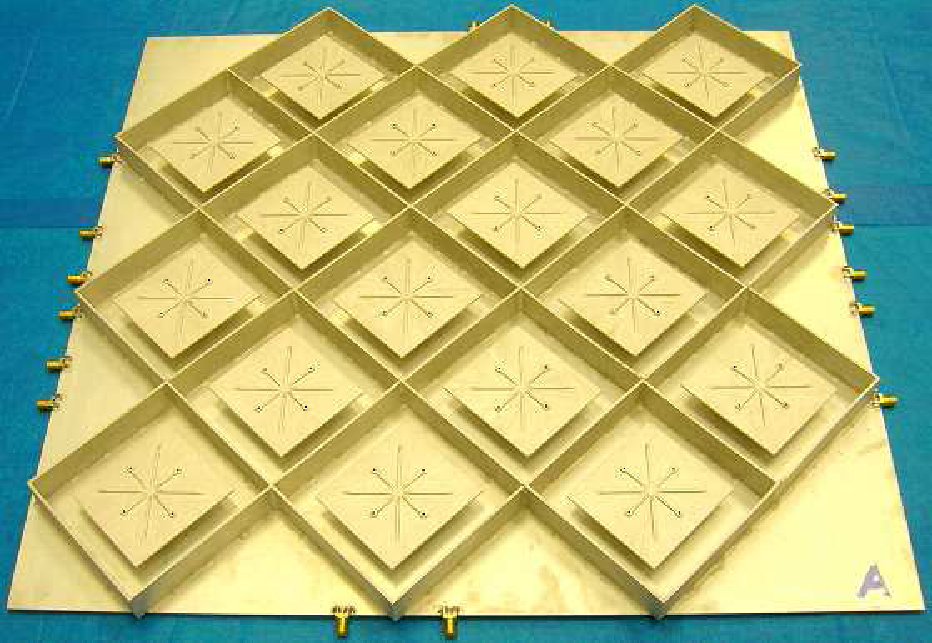
\includegraphics[width=4cm]{planArrayAlcatel} \\
%\tiny Active Antenna Arrays - Alcatel-Lucent Innovation Days � December 2008. BELL Labs Research Project
%\end{minipage}
%\end{minipage}
%\hspace{.1cm}
\begin{minipage}[l]{5cm}
%\begin{minipage}[t]{4cm}
\centering
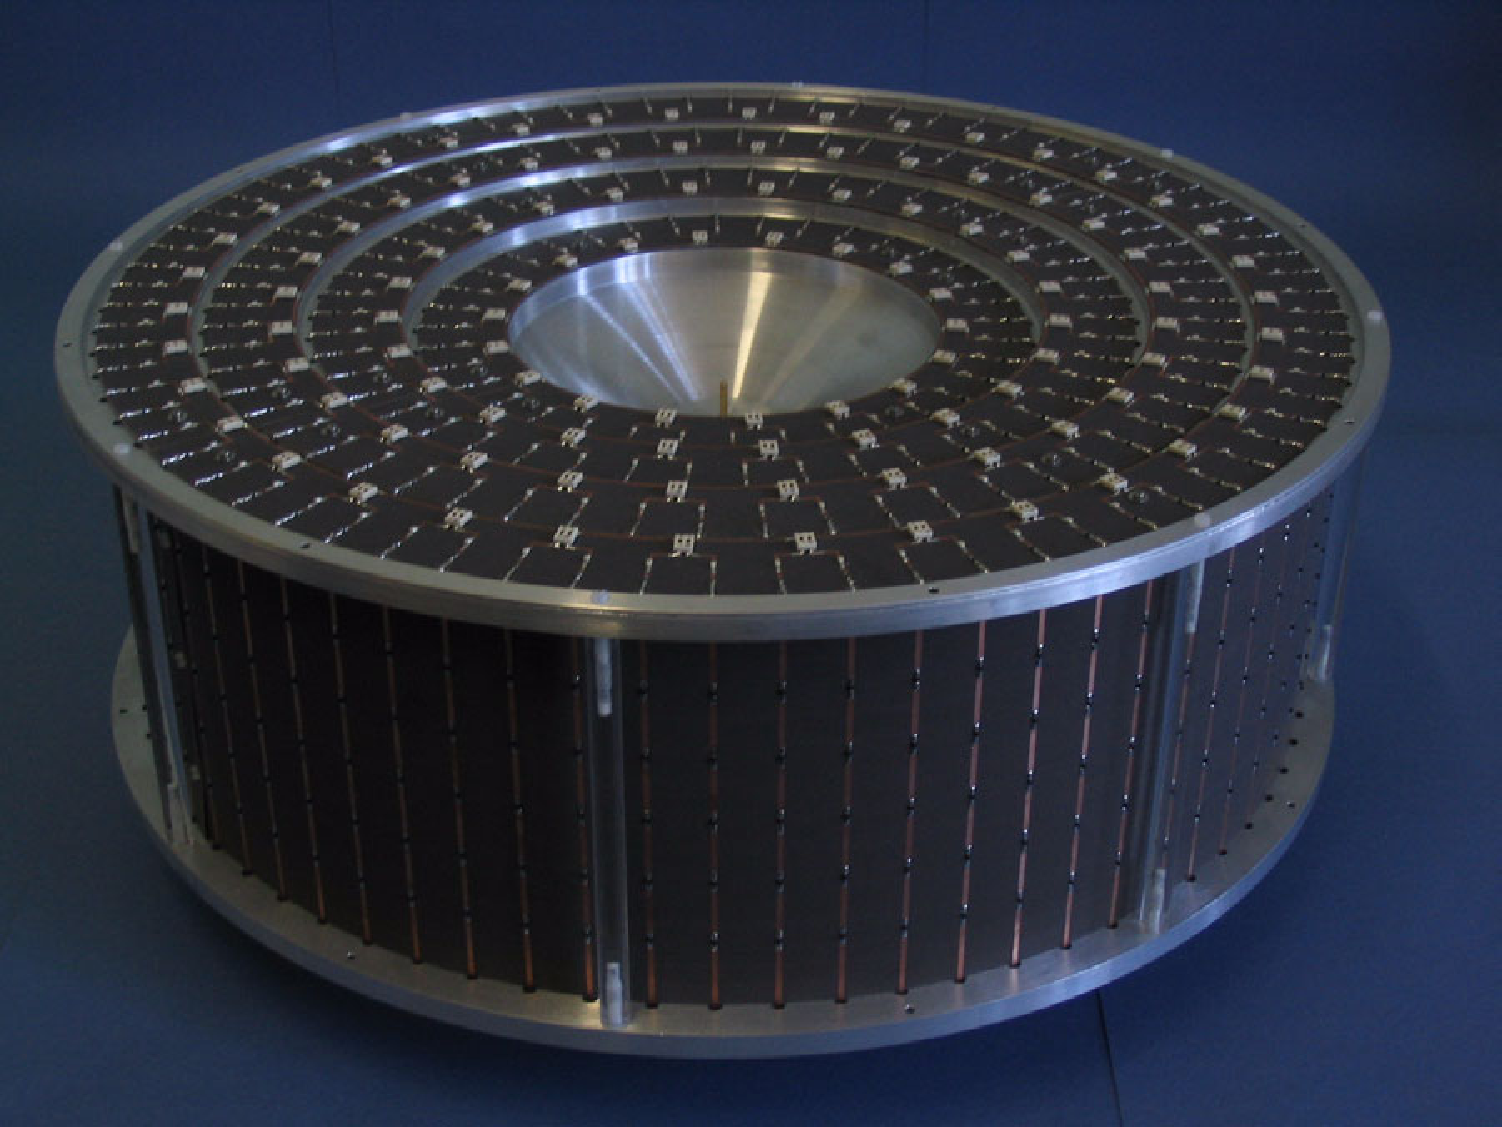
\includegraphics[width=5cm]{arrayEBG} \\
\tiny P. Ratajczak, P. Brachat, J.M. Fargeas, \quotes{Adaptive Beam Steering Base Station Antenna: Performances Optimization of the Reconfigurable EBG Material} - France Telecom
%\end{minipage}
%\begin{minipage}[b]{5cm}
%\centering
%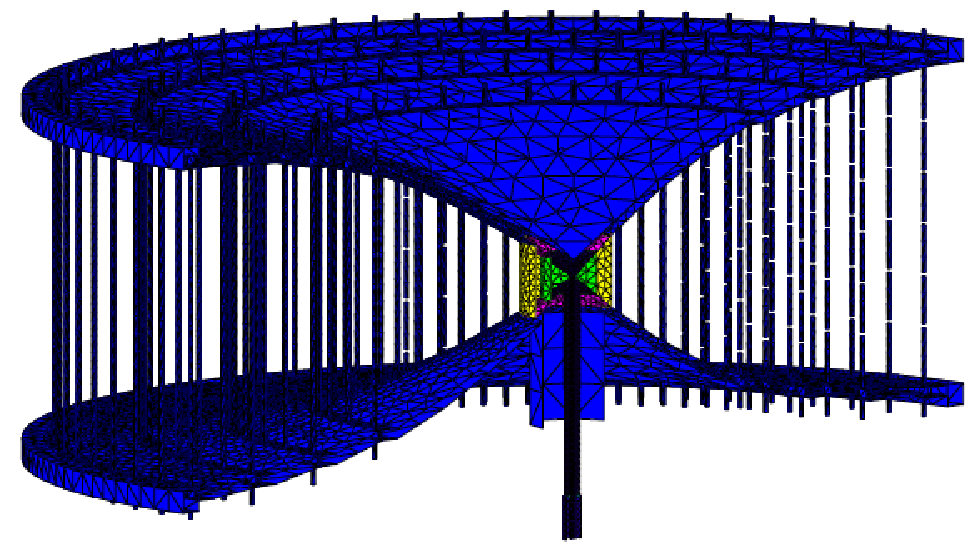
\includegraphics[width=4cm]{arrayEBGmod} \\
%\tiny P. Ratajczak, P. Brachat, J.M. Fargeas EBG Base Station Antenna Model
%\end{minipage}
%\centering
%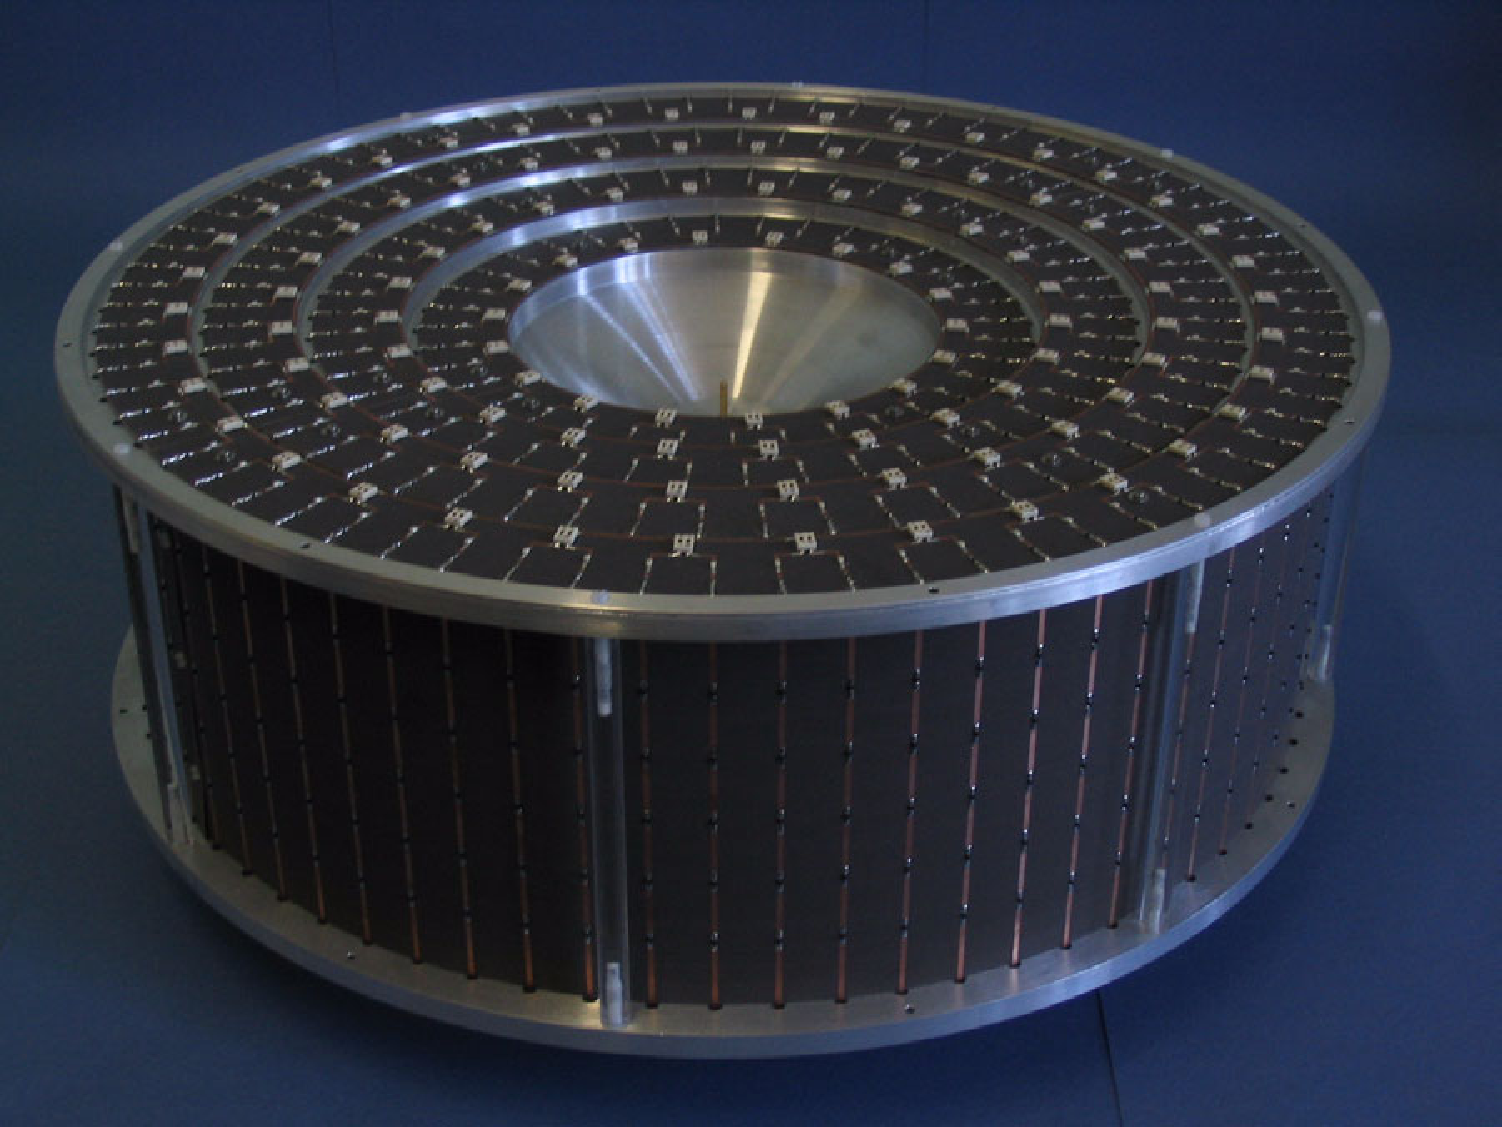
\includegraphics[width=5cm]{arrayEBG} \\
%\tiny Array planare di 12 x 16 dipoli ripiegati su supporto dielettrico
\end{minipage}
\end{figure}
\begin{pgfpicture}{0cm}{0cm}{0cm}{0cm}
 \pgfsetlinewidth{.25pt}%
% \pgfsetendarrow{\pgfarrowtriangle{2pt}}%
 \pgfline{\pgfxy(4.9,.6)}{\pgfxy(4.9,7)}
\end{pgfpicture}
}
\frame{
\frametitle{Analisi numerica di array fasati : criteri di analisi}
\begin{itemize}
	\item Flessibilit\acgrave{a} \\
	\begin{itemize}
		\item Geometria arbitraria degli elementi radianti \\
		\item Scelta arbitraria dei materiali \\
	\end{itemize}
\pause
	\item Elevata accuratezza ed affidabilit\acgrave{a} \\ 
	\begin{itemize}
		\item Soluzione \textsl{full-wave} delle equazioni di Maxwell \\
	\end{itemize}
\end{itemize} \pause
			\begin{center}
\vspace{-.3cm}
$\Downarrow$ \\[.1cm] Tecnica degli \alert{Elementi Finiti} (Sistema lineare) \\[.2cm] 
\pause
			%\hspace{1.3cm} (Sistema lineare) 
%\begin{itemize}
		Strutture elettricamente grandi $\Rightarrow$ \alert{ $\mbf{10^5}$ - $\mbf{10^{8}}$ incognite} !!! \\
		Soluzioni da calcolare per \alert{ciascuna direzione di scansione} !!! \\

%\end{itemize}
%\pause
\end{center}
%\vspace{-.2cm}
%\makebox[10cm]{
%\begin{colorblock}{mycolor}{mycolor}{}
%5\begin{center}
%	\acgrave{E} possibile \alert{ridurre la complessit\acgrave{a} del problema} mantenendo un adeguata accuratezza nel \itt{pattern} ? %  mantenendo un adeguata \alert{accuratezza nel \emph{pattern}} di radiazione al \alert{variare dell'angolo di scansione ?}
%\end{center} 
%\end{colorblock}
}

\subsection{Modello di radiazione e riduzione della complessit\acgrave{a}}
\frame{
\frametitle{Modello di radiazione e riduzione della complessit\acgrave{a}}
\begin{itemize}
%\item \alert{\itt{Pattern} di radiazione} (\itt{HPBW}, \textit{SLL}, polarizzazione, ...)
%\item Polarizzazione del campo radiato % (componenti co- e cross-polari)
%\item \alert{Mutui-accoppiamenti} tra elementi radianti (matrice di \itt{scattering}, eventuali angoli ciechi per strutture planari, ...) 
\item Vogliamo un \alert{modello di radiazione} che permetta, a seguito di una riduzione della complessit\acgrave{a},  di preservare le informazioni associate al \itt{pattern} di radiazione in scansione\\ \pause
\item \acgrave{E} necessario \alert{parametrizzare} tale modello, cio\acgrave{e} costruire un \alert{modello variabile nelle direzioni di scansione e in quelle di osservazione} che costituiscono il \itt{pattern} di radiazione


\end{itemize}
%\pause
%\begin{colorblock}{mycolor}{mycolor}{}
%\begin{center}

%\end{center} 
%\end{colorblock} \pause
%\begin{center}
%$\Downarrow$
%\end{center}
%\begin{colorblock}{mycolor}{mycolor}{}
%\begin{center}
%Diventa possibile andando a \alert{parametrizzare} il modello, creando quindi un \alert{modello variabile nelle direzioni di scansione e in quelle di osservazione} che costituiscono il \itt{pattern} di radiazione% nell'angolo di scansione}
%\end{center} 
%\end{colorblock}
}

\section{Modello di radiazione per array fasati}
\subsection{Tecnica degli elementi finiti}
\frame
{
  \frametitle{Formulazione Galerkin-Elementi finiti: campi vicini}
\scriptsize
\begin{columns}[cc]
\column{7cm}
\centering
Soluzione dell'\alert{equazione d'onda\\ per il campo elettrico}: \\[.2cm]
\alert{$\nabla \times \frac{1}{\mu_r} \nabla \times \mbfit{E} + jk_0\zeta_0\sigma \mbfit{E}  - k_0^2\epsilon_r \mbfit{E} = 0$} \\ $k_0 = \omega \sqrt{\epsilon_0 \mu_0}$, \ $\zeta_0 = \sqrt{\frac{\mu_0}{\epsilon_0}}$ \\[0.2cm]
nel dominio $\mrm{\Omega} \subset \mathbb{R}^3$ con contorno \\ $\mrm{\partial \Omega = \Gamma = \Gamma_E \cup \Gamma_{H} \cup \Gamma_{WG} \cup \Gamma_R}$ \\[.2cm] \pause
\begin{itemize}
 \item $\mrm{\Omega}_h = \bigcup_{m=1}^{M} \mrm{\Omega}_m \subset \mrm{\Omega}, \ \mrm{\Omega}_m \cap \mrm{\Omega}_n = \{ \varnothing \} \ \forall m \neq n $ \pause
 \item $\tilde{\mbfit{E}} := \sum_{j=1}^N e_j \mbfit{w}_j, \ \ \mbfit{w}_j \in \mathcal{W} \subset \mathcal{H}(\mrm{curl;\mrm{\Omega}})$ \pause
 \item Proiezione di Galerkin:% $\Rightarrow$ equazione differenziale in forma debole
\\[.1cm] \hspace{-.8cm}
 $\int_{\mrm{\Omega}_h} \mbfit{w}_i \cdot \left ( \nabla \times \frac{1}{\mu_r} \nabla \times \tilde{\mbfit{E}} + jk_0\zeta_0\sigma \tilde{\mbfit{E}}  - k_0^2\epsilon_r \tilde{\mbfit{E}} \right ) d\mrm{\Omega} = 0$ \\ \pause
\centering
\hspace{-1cm} $\Downarrow$ \\
\hspace{-1cm}
\begin{colorblock}{mycolor}{mycolor}{}
\normalsize $$\mat{A} \ \vect{e}_p  = \vect{b}_p, \qquad 1 \leq p \leq P$$
$$ \mat A \in \mathbb{C}^{N \times N}, \ \vect{b}_p, \vect{e}_p \in \mathbb{C}^{N \times 1}$$
\end{colorblock}
\end{itemize}
\column{5cm}
%\vspace{-1cm}
\begin{tabular*}{\textwidth}[]{c}
Maxwell nel dominio della frequenza:\\[.1cm]
$\nabla \times \mbfit E = -j \omega \mbfit B$ \\
$\nabla \times \mbfit H = j \omega \mbfit D + \sigma \mbfit E$ \\[.2cm]
Relazioni costitutive del mezzo: \\[.1cm]
$\mbfit D = \epsilon \mbfit E = \epsilon_r \epsilon_0 \mbfit E$\\
$\mbfit B = \mu \mbfit H = \mu_r \mu_0 \mbfit H$\\[.2cm]
\end{tabular*}
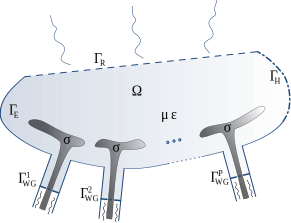
\includegraphics[width=5cm]{FEMproblem}
\end{columns}
}


\frame
{
\frametitle{Formulazione Galerkin-Elementi finiti: campi vicini}
\begin{itemize}
\item  $\vect{b}_p$  \acgrave{e} associato a $\mrm{\Gamma}^{p}_\mrm{WG}$ \ $\Rightarrow$ \ $\vect{e}_p  = \mat{A}^{-1} \ \vect{b}_p$ soluzioni per ciascuna delle $P$ porte di alimentazione dell'array \\[.1cm] Con il \alert{principio di sovrapposizione degli effetti} :\\[.1cm]
%\begin{center}
\hspace{-.3cm} $\displaystyle \left[ e_1, \dots , e_N \right]^T = \vect e = \sum_{p=1}^P \vect{e}_p$ %\\[.2cm]
\ \ \ \footnotesize  coefficienti di espansione per $\tilde{\mbfit{E}}$ \normalsize
%\end{center}
\vspace{.2cm} \pause
\item $\nabla \times {\mbfit{E}} =  -j\omega{\mbfit{B}}$ \ \ $\Rightarrow$ \ \ $\tilde{\mbfit H} = - \frac{1}{j \omega \mu} \nabla \times \tilde{\mbfit E}$ \vspace{.2cm} \pause
\item Dominio computazionale $\mrm {\Omega}_h$ \acgrave{e} ristretto ai \alert{campi vicini}, che ne \acgrave{e} dei \alert{campi radiati} ?%, quindi del \alert{\itt{pattern} di radiazione} ?
\end{itemize}
}

\subsection{Trasformazione da campi vicini a campi lontani}
\frame
{
\frametitle{Trasformazione da campi vicini a campi lontani}
\begin{itemize}
\item \alert{Principio di Huygens}: campi lontani derivati dai campi vicini $\tilde{\mbfit{E}}=\tilde{\mbfit{E}}(\mbfit{r'})$ e $\tilde{\mbfit{H}}=\tilde{\mbfit{H}}(\mbfit{r'})$, $\mbfit{r'} \in \mrm{\Gamma_R}$
% dalle correnti equivalenti} ${\mbfit{J}}_s^{eq} = \hat{\mbfit{n}} \times \tilde{\mbfit{H}}$ e ${\mbfit{J}}_{ms}^{eq} = - \hat{\mbfit{n}} \times \tilde{\mbfit{E}}$ calcolate su $\mrm{\Gamma_R}$\\[.2cm]
%\hspace{-.5cm}
\begin{center}
\vspace{-.5cm} \scriptsize $$\hspace{-.5cm}\check{\mbfit{E}}(\theta, \phi) = j \frac{\zeta_0 k_0}{4 \pi} \int \! \! \! \! \int_\mrm{\Gamma_R}  \mrm{e}^{jk_0 \hat{\mbfit{r}} \cdot \mbfit{r'}} \left [ - (\hat{\mbfit{n}} \times \tilde{\mbfit{H}})  + \left ( ( \hat{\mbfit{n}} \times \tilde{\mbfit{H}} ) \cdot \hat{\mbfit{r}} \right ) \hat{\mbfit{r}} + \frac{1}{\zeta_0} \ (\hat{\mbfit{n}} \times \tilde{\mbfit{E}})  \times \hat{\mbfit{r}} \right ]  d{\Gamma}$$ \vspace{-.2cm} \footnotesize $$ \hat{\mbfit{r}} = \hat{\mbfit{r}} \left ( \theta, \phi \right ) \textnormal{ versore nella \alert{direzione di osservazione}}$$ \vspace{-.5cm} $$\hat{\mbfit{n}} \textnormal{ normale su } \mrm{\Gamma_R} \textnormal{ uscente da } \mrm{\Omega}_h $$
\end{center} %  \\[.3cm] 
%\vspace{.2cm} 
\pause
\item \normalsize \alert{Approssimazione per campi radiati}: $\check{\mbfit{H}}(\theta, \phi) =  \frac{1}{\zeta_0} \hat{\mbfit{r}} \times \check{\mbfit{E}}(\theta, \phi )$ \\ \pause % ci permette di trascurare il campo magnetico 
%\vspace{.2cm}
%\pause
%\item \alert{Potenza radiata}: \vspace{-.2cm} $$\mrm{P}_\mrm{rad} = \frac{1}{2} \Re \left \{ \int_{\mrm{\Gamma_R}} \left [ \tilde{\mbfit{E}} \times \tilde{\mbfit{H}}^{*} \right ] \cdot \hat{\mbfit{n}} \ d\mrm{\Gamma} \right \}  = \mrm{P}_\mrm{in} - (\mrm{P}_\mrm{rifl} + \mrm{P}_\mrm{diss})$$ \\ \pause
\item \alert{\itt{Pattern} di radiazione}: \vspace{-.2cm}
$$\mrm{G}_{\hat{\theta}} \left ( \theta, \phi \right ) = 4 \pi \frac{\left | {{\hat{\theta}}} \cdot \check{\mbfit E} (\theta, \phi) \right |^2}{ 2 \zeta_0 \mrm{P}_\mrm{acc}}, \ \mrm{G}_{\hat{\phi}} \left ( \theta, \phi \right ) = 4 \pi \frac{\left | {\hat{\phi}} \cdot \check{\mbfit E} (\theta , \phi ) \right |^2}{ 2 \zeta_0 \mrm{P}_\mrm{acc}}$$ \\[-.2cm]
$$\mrm{G}_{tot} \left ( \theta, \phi \right )  = \mrm{G}_{\hat{\theta}} \left ( \theta, \phi \right ) + \mrm{G}_{\hat{\phi}} \left ( \theta, \phi \right ) $$
\vspace{-.2cm} \footnotesize $$\mrm{P_{acc}} = \mrm{P_{inc}} - \mrm{P_{rifl}}  \textnormal{: potenza accettata dalle }P\textnormal{ porte di alimentazione}$$ 

\end{itemize}
}

\subsection{Sistema lineare tempo-invariante}
\frame
{
\frametitle{Modello di radiazione: relazione Ingresso-Stato}
%\only<1>{\vspace{-1.46cm}}
%\only<2>{\vspace{.02cm}}
\begin{itemize}
%\item $\mat{A} \ \vect{e}_p  = \vect{b}_p$ \ $\Leftrightarrow$ \ \alert{relazione Ingresso-Stato} di un sistema lineare tempo-invariante%. Le incognite del sistema costituiscono un \alert{vettore di stato} 
%\only<2>{\\[.15cm]}
%\pause
\item $\mat{A} \ \vect{e}_p  = \vect{b}_p$ + \alert{fasori di eccitazione} per interferenza costruttiva nella direzione di scansione $(\theta_s,\phi_s)$: \vspace{-.2cm}
$$\xi_p(\theta_s,\phi_s) = \mrm{e}^{-jk_0 ( x_p \sin(\theta_{s}) \cos(\phi_s) + y_p \sin(\theta_{s}) \sin(\phi_s) + z_p \cos(\theta_s) )}$$ %\only<1>{\\[-.2cm]} 
\footnotesize $(x_p,y_p,z_p)$ posizione del $p$-esimo elemento radiante di un array generico \\ \pause % disposto sul piano XY\\
\item \normalsize \alert{Relazione Ingresso-Stato parametrizzata nella direzione di scansione $(\theta_s,\phi_s)$} \\ 
\begin{colorblock}{mycolor}{mycolor}{}
$$\mat{A} \ \vect{e} (\theta_s,\phi_s)  = \sum_{p=1}^{P} \xi_p(\theta_s,\phi_s) \ \vect{b}_p $$ %u(\theta_s,\phi_s)
\end{colorblock}
\end{itemize}
%\begin{center}
%\only<2>{\vspace{-.5cm} 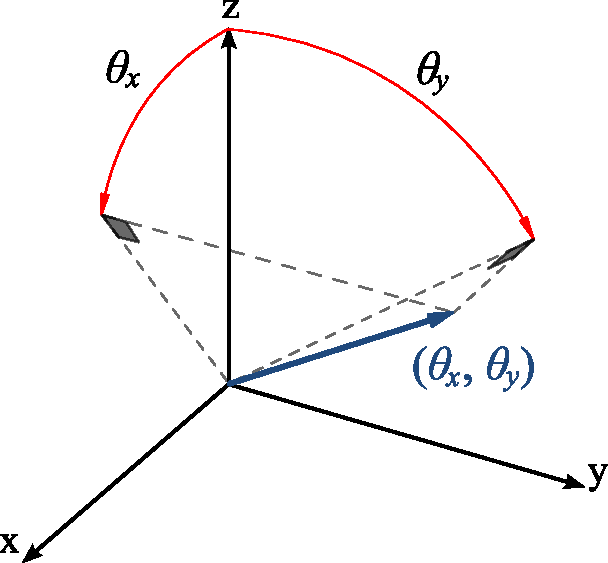
\includegraphics[width=4cm]{scanAngles}}
%\end{center}
}

%\frame
%{
%\frametitle{Modello di radiazione: relazione Ingresso-Stato}
%\begin{itemize}
%\item \normalsize \alert{Relazione Ingresso-Stato parametrizzata nella direzione di scansione $(\theta_s,\phi_s)$} \\ 
%\begin{colorblock}{mycolor}{mycolor}{}
%$$\mat{A} \ \vect{e} (\theta_s,\phi_s)  = \sum_{p=1}^{P} \xi_p(\theta_s,\phi_s) \ \vect{b}_p $$ %u(\theta_s,\phi_s)
%\end{colorblock}
%\end{itemize}
%}

\frame
{
\frametitle{Modello di radiazione: relazione Stato-Uscita}
\begin{itemize}
\item Relazione integrale che lega i campi vicini al campo elettrico radiato \ $\Rightarrow$ \ \alert{operatori sui campi vicini} per le polarizzazioni in ${\hat{\theta}}$ e ${\hat{\phi}}$ dei campi radiati \vspace{-.1cm} $$ \check{\mbfit E}_{\hat{\theta}} (\theta, \phi) = {\hat{\theta}} \cdot \check{\mbfit E} (\theta, \phi) = {\mathcal{L}}_{\hat{\theta}}(\tilde{\mbfit E}, \tilde{\mbfit H} ; \theta, \phi)$$ \\[-.6cm] $$ \check{\mbfit E}_{\hat{\phi}} (\theta, \phi) = {\hat{\phi}} \cdot \check{\mbfit E} (\theta, \phi) = {\mathcal{L}}_{\hat{\phi}}(\tilde{\mbfit E}, \tilde{\mbfit H} ; \theta, \phi)$$ \pause
\vspace{-.5cm}
%\item Per poter ridurre la complessit\acgrave{a} del sistema \ $\Rightarrow$ \ forma parametrizzata della relazione di Stato-Uscita \pause
\item Espressione degli operatori, per piani a $\phi$ costante, in \alert{serie di Fourier complessa} \\[-.6cm]
$$\hspace{-.8cm} \mathcal{L}_{\{ {\hat{\theta}},{\hat{\phi}} \}}(\tilde{\mbfit E}, \tilde{\mbfit H}; \theta, \phi |_\mrm{cost}) = \sum_{q=-\infty}^{\infty} k_{q \{ {\hat{\theta}},{\hat{\phi}} \}} (\tilde{\mbfit E}, \tilde{\mbfit H} ; \phi |_\mrm{cost}) \ \eta_q(\theta)$$
\vspace{-.2cm} $$\displaystyle \eta_q(\theta) = \mrm{e}^{\ j q \theta}, \ -\infty \leq q \leq \infty$$
\end{itemize}
}

\frame
{
\frametitle{Modello di radiazione: relazione Stato-Uscita}
\centering
\vspace{-.1cm}
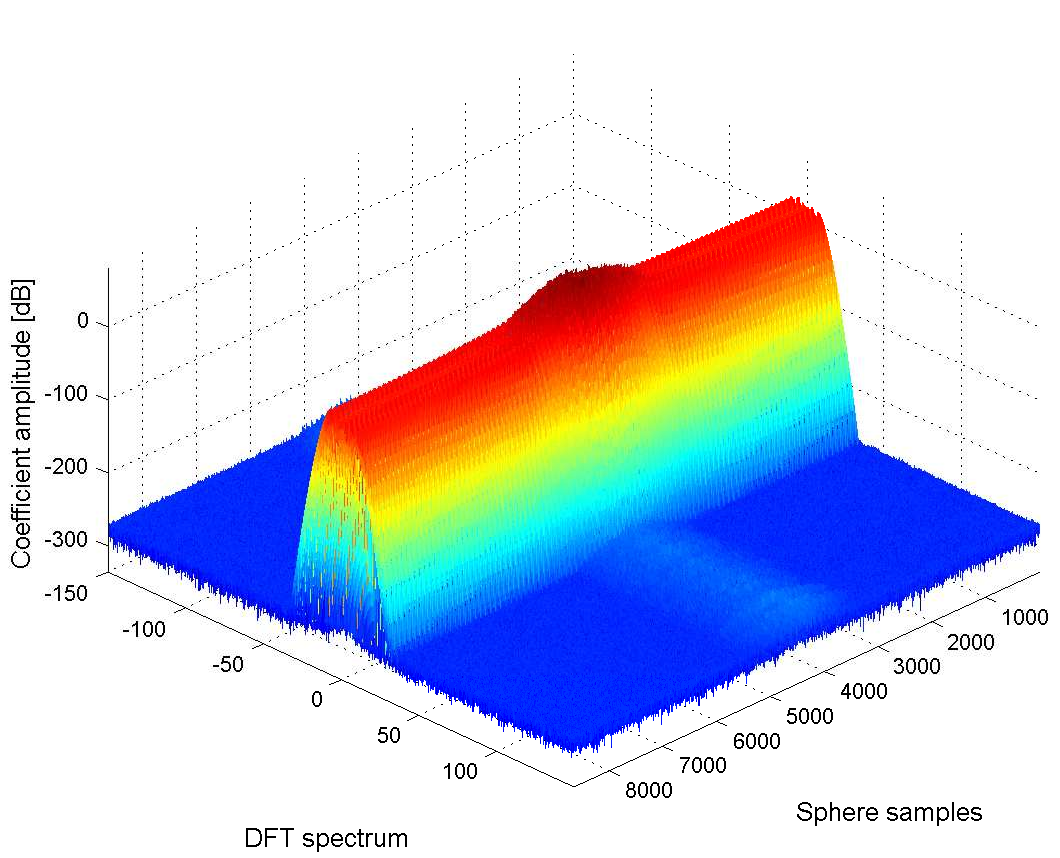
\includegraphics[width=6.5cm]{DFTspectrum}
\begin{itemize}
\item Lo spettro degli operatori \acgrave{e} a banda stretta \ $\Rightarrow$ \ \alert{\itt{DFT-truncation}} ai $2Q+1$ principali termini della serie di Fourier \\[-.6cm] \footnotesize
$$\hspace{-.9cm} {\mathcal{L}}_{\{ {\hat{\theta}},{\hat{\phi}} \}}(\tilde{\mbfit E}, \tilde{\mbfit H}  ; \theta, \phi |_\mrm{cost}) \approx \tilde{\mathcal{L}}_{\{ {\hat{\theta}},{\hat{\phi}} \}}(\tilde{\mbfit E}, \tilde{\mbfit H}  ; \theta, \phi |_\mrm{cost}) = \sum_{q=-Q}^{Q} k_{q \{ {\hat{\theta}},{\hat{\phi}} \}} (\tilde{\mbfit E}, \tilde{\mbfit H} ; \phi 
|_\mrm{cost}) \ \eta_q(\theta)$$
\end{itemize}
}

\frame
{
\frametitle{Modello di radiazione: relazione Stato-Uscita}
\begin{itemize}
\item $\qquad \qquad \tilde{\mbfit E} = \mathcal{F}_{\tilde{\mbfit E}}( \vect e (\theta_s,\phi_s))$, $\tilde{\mbfit H} = \mathcal{F}_{\tilde{\mbfit H}}( \vect e (\theta_s,\phi_s))$ su $\mrm{\Gamma_R}$\\[-.4cm] $$\Downarrow$$ \\[-.8cm]
%\footnotesize
$$ \check{\mbfit E}_{\{ {\hat{\theta}},{\hat{\phi}} \}} (\theta, \phi |_\mrm{cost}) \approx \tilde{\mathcal{L}}_{\{ {\hat{\theta}},{\hat{\phi}} \}} \left ( \mathcal{F}_{\tilde{\mbfit E}}( \vect e (\theta_s,\phi_s)), \mathcal{F}_{\tilde{\mbfit H}}( {\vect e} (\theta_s,\phi_s)) ; \theta, \phi |_\mrm{cost} \right ) $$ \pause
%\item \itt{DFT-truncation} (${\mathcal{L}}_\theta \approx \tilde{\mathcal{L}}_\theta$, ${\mathcal{L}}_\phi \approx \tilde{\mathcal{L}}_\phi$) $\Rightarrow$
%\normalsize
\item \alert{Relazione Stato-Uscita parametrizzata nella direzione di osservazione $(\theta, \phi |_\mrm{cost})$}\\
\begin{colorblock}{mycolor}{mycolor}{}
$$ \check{\mbfit E}_{\{ {\hat{\theta}},{\hat{\phi}} \}}(\theta, \phi |_\mrm{cost}) =  \left ( \sum_{q=-Q}^{Q} \eta_q(\theta) \ \vect{c}^H_{q\{ {\hat{\theta}},{\hat{\phi}} \}}(\phi |_\mrm{cost}) \right ) \ \vect{e} (\theta_s,\phi_s)$$
$$\vect{c}_{q\{ {\hat{\theta}},{\hat{\phi}} \}}(\phi |_\mrm{cost}) \in \mathbb{C}^{N \times 1}$$
\end{colorblock}
\end{itemize}
}
\frame
{
\frametitle{Sistema Ingresso-Stato-Uscita completo}
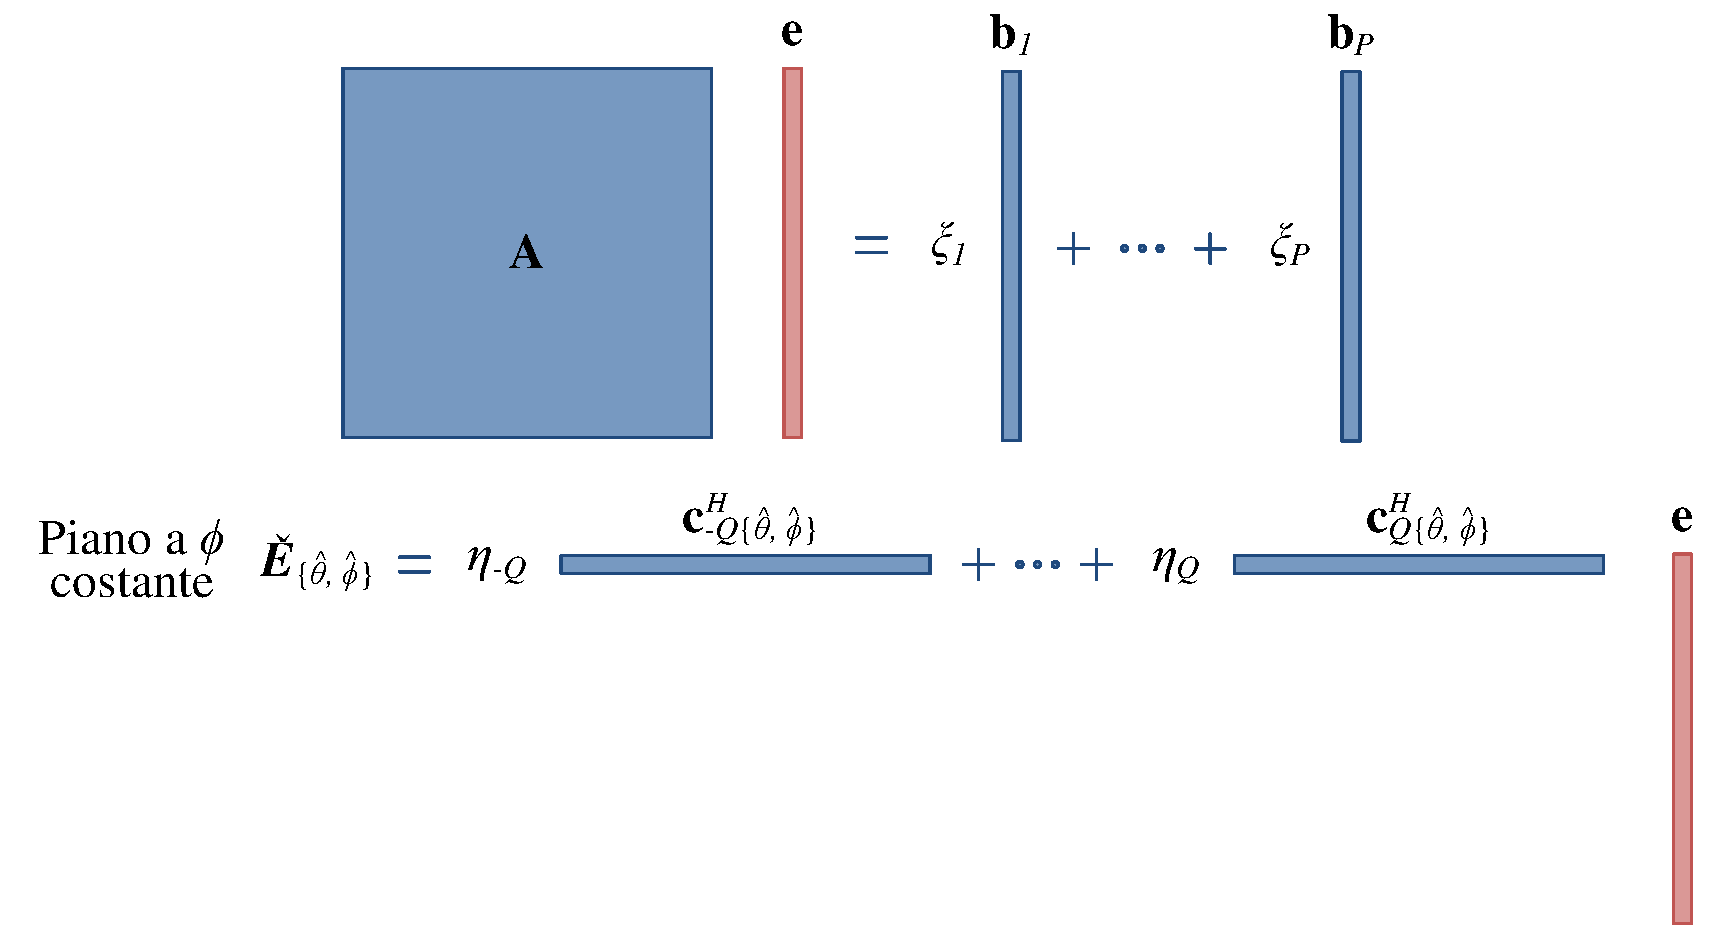
\includegraphics[width=\textwidth]{FullRadModel}
}

\subsection{Riduzione della complessit\acgrave{a}}
\frame
{
\frametitle{Sistema Ingresso-Stato-Uscita completo: proiezione}
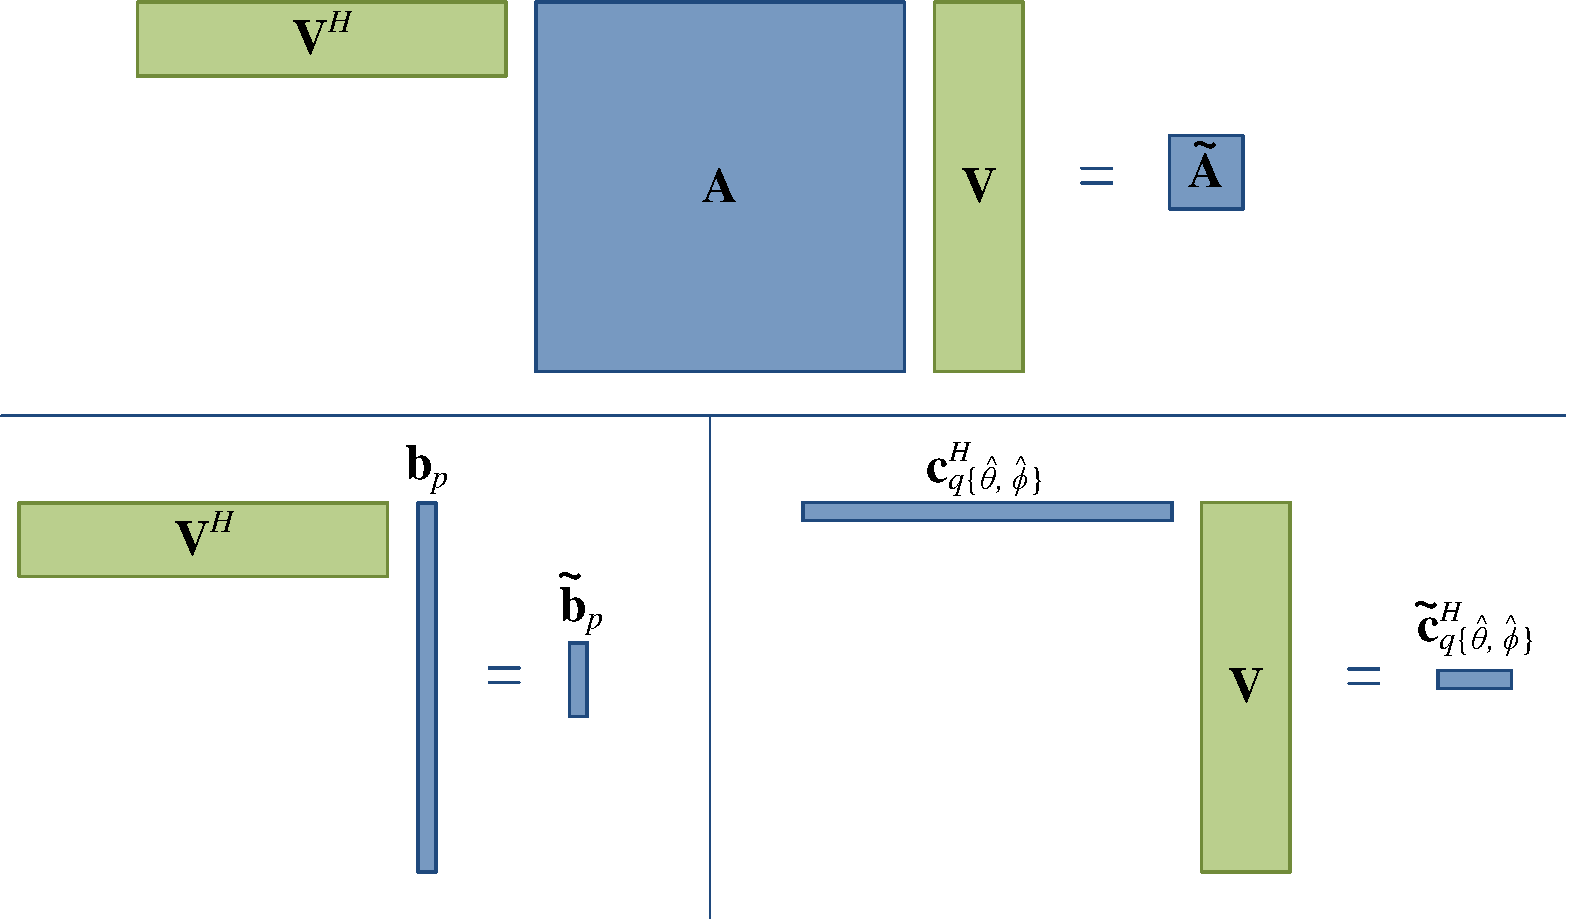
\includegraphics[width=\textwidth]{ROMproj}
$$\small \mat{V} \in \mathbb{C}^{N \times n}, \ n \ll N$$
}


\frame
{
\frametitle{Sistema Ingresso-Stato-Uscita ridotto}
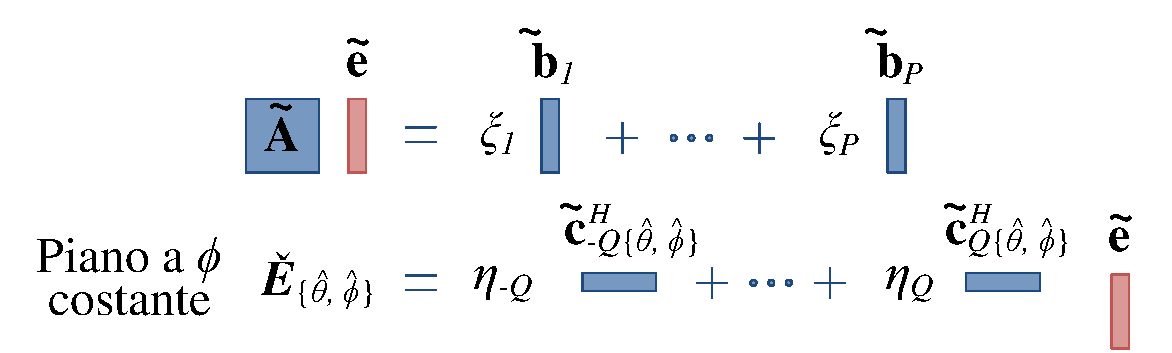
\includegraphics[width=\textwidth]{ROM}
%\begin{center}
%\vspace{-.7cm}
%\begin{eqnarray*}
%\label{eq:ROMSISO}
%\tilde{\mat{A}} \ \tilde{\vect{e}} (\theta_s,\phi_s) & = & \sum_{p=1}^{P} %\xi_p(\theta_s,\phi_s) \ \tilde{\vect{b}}_p  \\ %u(\theta_s,\phi_s) \\
% \check{\mbfit E}_{\{\theta,\phi\}}(\theta, \phi |_\mrm{cost}) & = & \left ( %\sum_{q=-Q}^{Q} \eta_q(\theta) \ \tilde{\vect{c}}^H_{q\{\theta,\phi\}}(\phi %|_\mrm{cost}) \right ) \ \tilde{\vect{e}} (\theta_s,\phi_s) \\
%\vect{z}(\theta_s,\phi_s) &= & \tilde{\mat F} \ \tilde{\vect{e}} %(\theta_s,\phi_s)
%\end{eqnarray*} con
%\begin{eqnarray*}
%\label{eq:ProjectedSISO}
%\tilde{\mat{A}} & := & \mat{W}^H \ \mat{A} \ \mat{V} \\
%\tilde{\vect{b}}_p & := & \mat{W}^H \ \vect{b}_p \\
%\tilde{\vect{c}}_{q\{\theta,\phi\}} & := & \mat{V}^H \ %\vect{c}_{q\{\theta,\phi\}} \\
%\tilde{\mat{F}}& := & \mat{F} \ \mat{V}
%\end{eqnarray*} e $\mat{W}, \mat{V} \in \mathbb{C}^{N \times n}, \ n \ll N$
%\end{center}
}

\frame{
\frametitle{Sottospazio di proiezione}
\begin{itemize}
\item $\mat V$ costituisce una \alert{base} di espansione del vettore delle soluzioni $\tilde{\vect e}(\theta_s,\phi_s)$: $\vect e(\theta_s,\phi_s) \approx \mat V \tilde{\vect e}(\theta_s,\phi_s)$ $\Rightarrow$ \alert{ $\mat V$ deve contenere informazioni sul campo vicino in scansione} \\ \pause 
%\item $\mat W$ costituisce uno \alert{spazio di \itt{test}} per la relazione Ingresso-Stato \pause
%\pause
%\begin{itemize}
\item \alert{Collezione di $\alpha$ soluzioni} linearmente indipendenti per direzioni di scansione $(\theta_{s_i}, \phi_{s_i})$, $1 \leq i \leq \alpha$ $\Rightarrow$ \alert{processo di ortonormalizazzione} $\Rightarrow$ $\mat V$
$$\mrm{span} \ \left \{ \bigcup_{i=1}^\alpha  \ \vect{e}_i(\theta_{s_i}, \phi_{s_i}) \right \} \subseteq \colspan{\mat V}$$\\ \pause
%\item Proiezione di Galerkin: $\mat W = \mat V$ $\Rightarrow$ \itt{matching} negli direzioni di scansione selezionati $(\theta_{s_i}, \phi_{s_i})$ 
%\item Emisfero settentrionale \ $\Rightarrow$ \ $\theta_{s_i}, \phi_{s_i} \in [-90\�,90\�]$ \\ 
%\pause
\item L'\alert{errore di riduzione della complessit\acgrave{a}} si calcola come errore $\varepsilon$ indotto al \itt{pattern} nella norma $\mathcal{L}^2$:
$$\varepsilon = \frac{\| \mrm{G}_{{tot}_{completo}} - \mrm{G}_{{tot}_{ridotto}} \|_2}{\| \mrm{G}_{{tot}_{completo}} \|_2}$$
%\end{itemize}
\end{itemize}
%\begin{colorblock}{mycolor}{mycolor}{}
%\begin{center}
%\alert{$\alpha$} ?
%\end{center}
%\end{colorblock}
}
%\frame{
%\frametitle{Analisi del campo vicino in \textbf{scansione lineare} - campo scalare $\psi$}
%\begin{itemize}
%\item $\displaystyle \mrm{span} \ \left \{ \bigcup_{i=1}^\alpha  \ \mbfit{\psi}_i(\theta_{s_i}, \phi_{s_i}) \right \} \subseteq \colspan{\mat V}, \ \alpha = 1, 2, 3, \ldots$ \pause
%\item Proiezione di $\mbfit{\psi}_t(\theta_{s_t},\phi_{s_t}) \neq \mbfit{\psi}_i(\theta_{s_i},\phi_{s_i}), 1 \leq i \leq \alpha$ nel sottospazio espanso da $\mat V$:\\ \vspace{-.4cm} $$\tilde{\mbfit{\psi}}_t = \mat{V} \mat{V}^H \mbfit{\psi}_t $$\\[-.6cm] \pause
%\item Valutazione dell'\alert{errore di approssimazione} (norma $\mathcal{L}^2$):\vspace{-.2cm} $$\color{blue} \varepsilon_\mrm{vicino} \color{black} = \frac{\|\mbfit{\psi}_t - \tilde{\mbfit{\psi}}_t \|_2}{\| \mbfit{\psi}_t \|_2}$$ \\[-.9cm]
%$$\color{red}  \varepsilon_\mrm{trasformato} \color{black} = \frac{\|\check{\mbfit{\psi}}_{t_\mrm{trasf.}} - \tilde{\check{\mbfit{\psi}}}_t \|_2}{\| \check{\mbfit{\psi}}_{t_\mrm{trasf.}} \|_2}$$ \\[-.7cm]
%$$\color{black} \varepsilon_\mrm{diretto}  = \frac{\| \check{\mbfit{\psi}}_{t_\mrm{dir.}} - \tilde{\check{\mbfit{\psi}}}_t \|_2}{\| \check{\mbfit{\psi}}_{t_\mrm{dir.}} \|_2}$$
%\end{itemize}
%}

%\frame{
%\frametitle{Analisi del campo vicino in \textbf{scansione lineare} - campo scalare $\psi$}
%\begin{center}
%\vspace{-.4cm}
%Array lineare di 17 sorgenti puntiformi disposte lungo $x$\\
%$\theta_{s_i} \in \{0\�, 90\�, 45\�, 22.5\�, 67.5\�, \ldots \}, \ \phi_{s_i} = 0\�, \ 1 \leq i \leq \alpha$
%\end{center}
%\vspace{.2cm}
%\hspace{-.5cm}\alert{$\Delta x = \nicefrac{\lambda}{4}$}\\[.3cm]
%\scriptsize{\hspace{-.5cm}Risoluzione nel \\\hspace{-.7cm} campionamento \\
%\hspace{-.6cm} di $\psi \approx \nicefrac{\lambda}{10}$}
%\begin{center}
%\vspace{-2.005cm}
%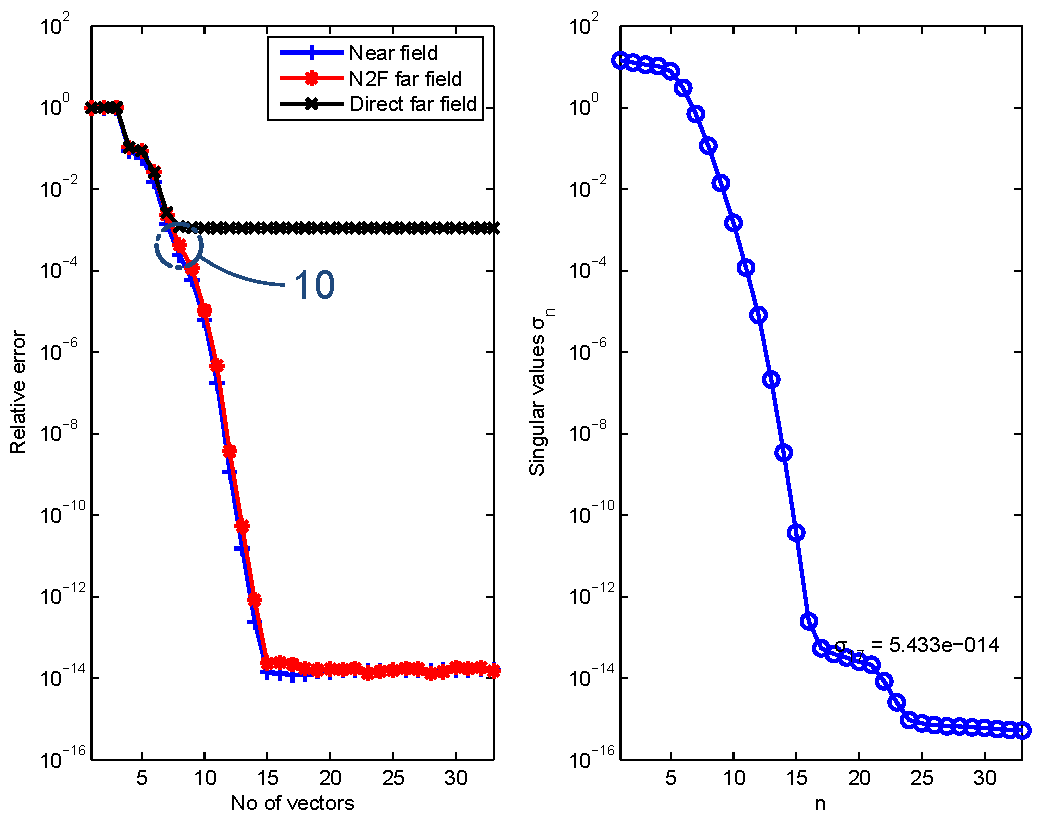
\includegraphics[width=7.5cm]{SVDerrorExp_33_0,25}
%\end{center}
%\begin{pgfpicture}{0cm}{0cm}{0cm}{0cm}
% \pgfsetlinewidth{.75pt}%
% \pgfsetendarrow{\pgfarrowtriangle{2pt}}%
% \pgfline{\pgfxy(1.5,4.88)}{\pgfxy(2.7,4.88)}
%\end{pgfpicture}
%}

%\frame{
%\frametitle{Analisi del campo vicino in \textbf{scansione lineare} - campo scalare $\psi$ }
%\begin{center}
%\vspace{-.4cm}
%Array lineare di 17 sorgenti puntiformi disposte lungo $x$\\
%$\theta_{s_i} \in \{0\�, 90\�, 45\�, 22.5\�, 67.5\�, \ldots \}, \ \phi_{s_i} = 0\�, \ 1 \leq i \leq \alpha$
%\end{center}
%\vspace{.2cm}
%\hspace{-.5cm}\alert{$\Delta x = \nicefrac{\lambda}{2}$}\\[.3cm]
%\begin{center}
%\vspace{-.8cm}
%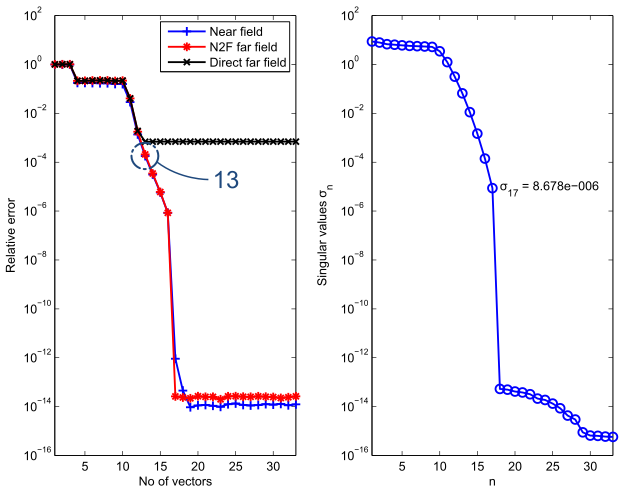
\includegraphics[width=7.5cm]{SVDerrorExp_33_0,5}
%\end{center}
%}

%\frame{
%\frametitle{Analisi del campo vicino in \textbf{scansione lineare} - campo scalare $\psi$}
%\begin{center}
%\vspace{-.4cm}
%\only<2>{\vspace{-.337cm}}
%Array lineare di 17 sorgenti puntiformi disposte lungo $x$\\
%$\theta_{s_i} \in \{0\�, 90\�, 45\�, 22.5\�, 67.5\�, \ldots \}, \ \phi_{s_i} = 0\�, \ 1 \leq i \leq \alpha$
%\end{center}
%\vspace{.2cm}
%\only<2>{\vspace{-.2cm}}
%\hspace{-.5cm}\alert{$\Delta x = \nicefrac{3 \lambda}{4}$}\\[.3cm]
%\begin{center}
%\vspace{-.8cm}
%\vspace{-.8cm}
%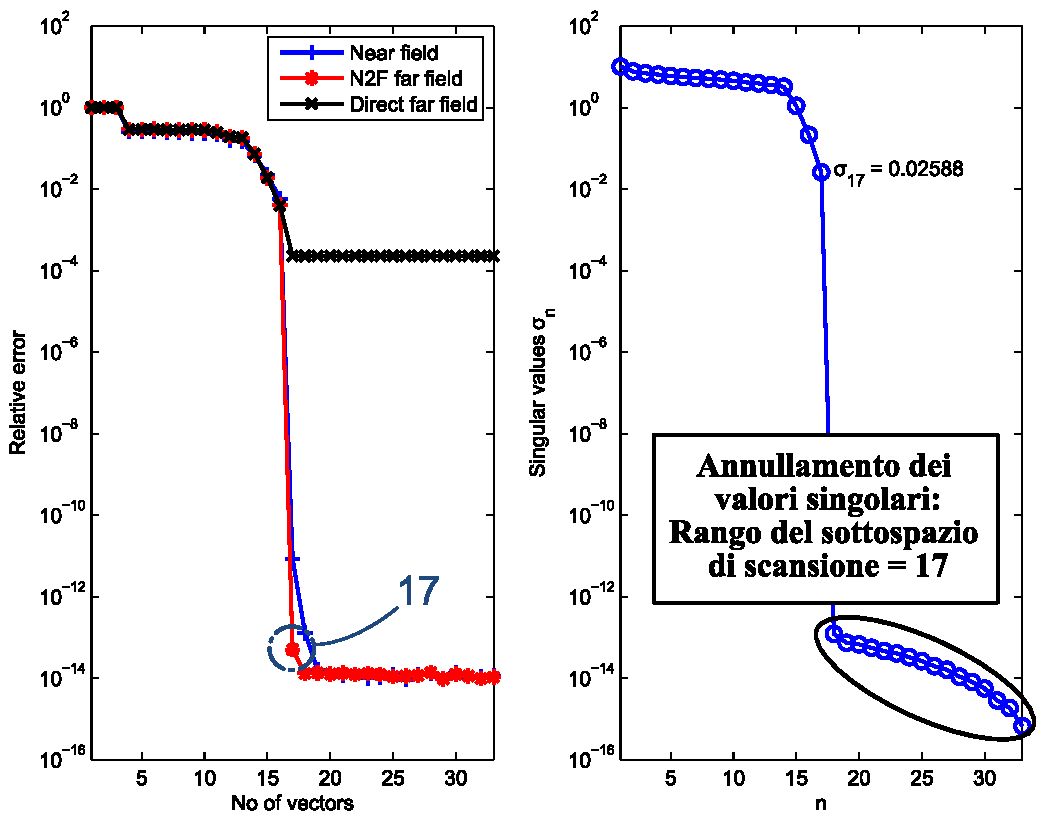
\includegraphics[width=7.5cm]{SVDerrorExp_33_0,75}
%\only<1>{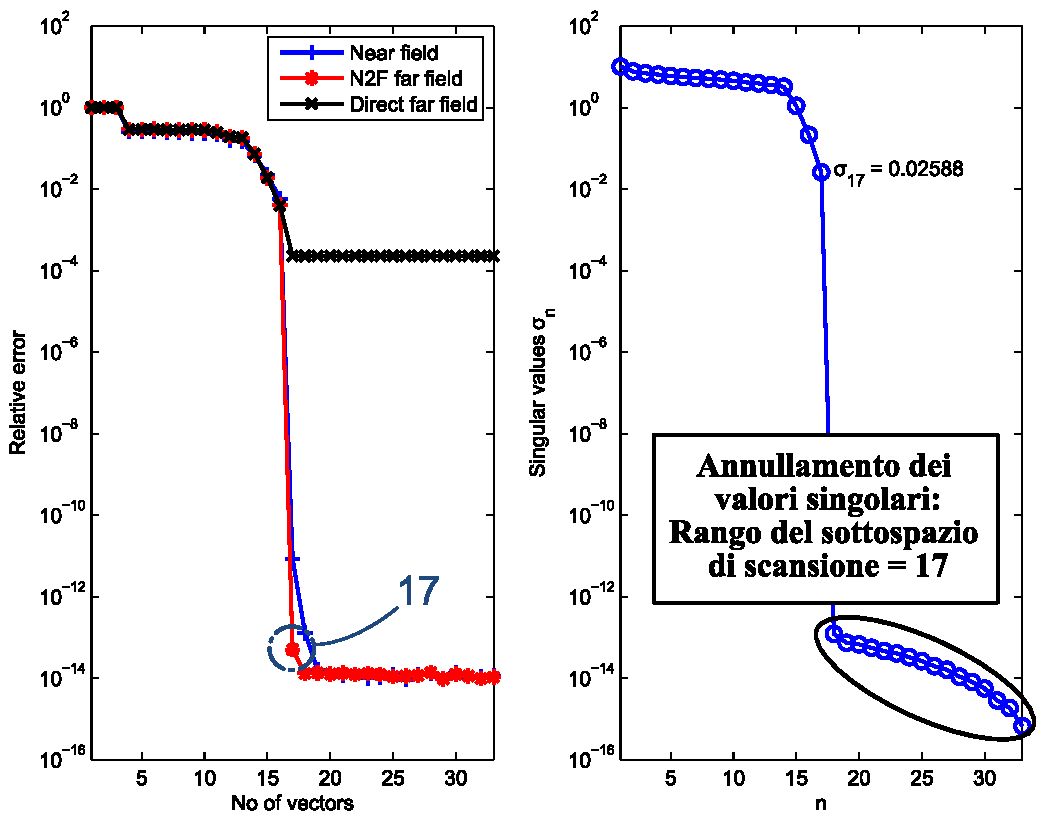
\includegraphics[width=7.5cm]{SVDerrorExp_33_0,75}}
%\only<2>{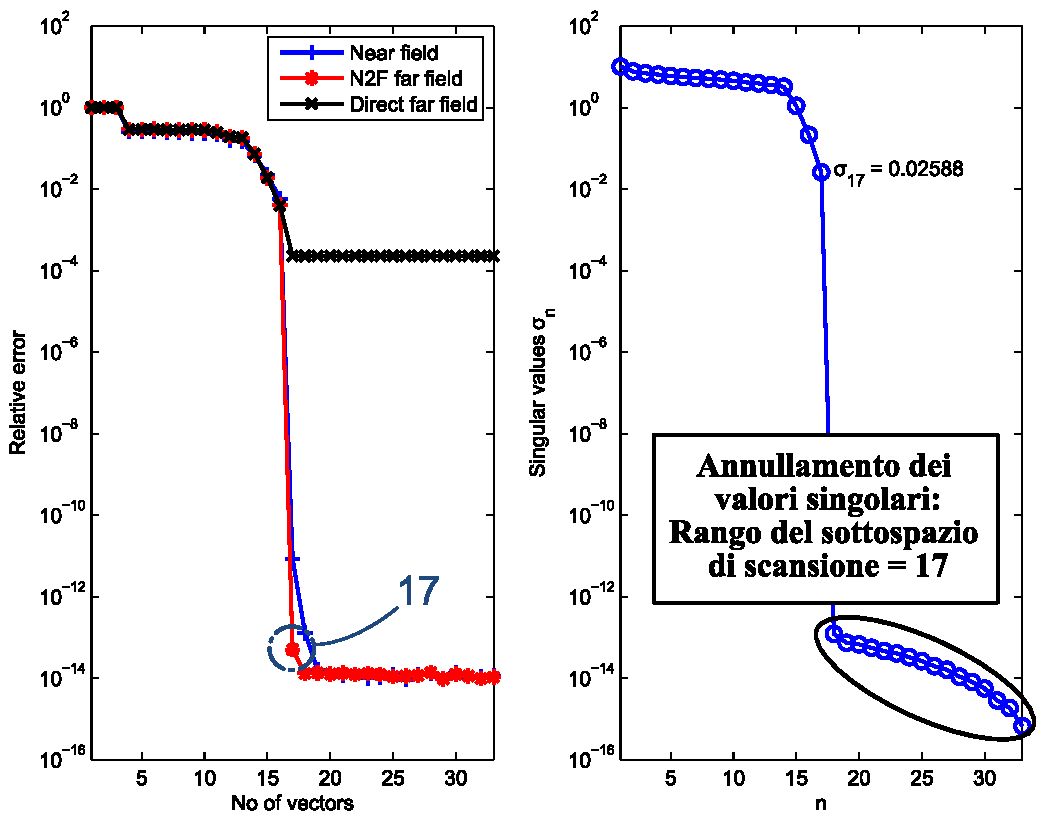
\includegraphics[width=5.5cm]{SVDerrorExp_33_0,75}}
%\end{center}
%\pause
%\begin{itemize}
%\only<2>{
%\begin{colorblock}{mycolor}{mycolor}{}
%\vspace{-.5cm}
%$\alpha$ in \alert{scansione lineare} dipende dal \alert{numero di elementi radianti} (rango del sottospazio di scansione) e dalle loro \alert{distanze relative}% pause
%\end{colorblock}
%}
%}

%\frame{
%\frametitle{Analisi del campo vicino in scansione lineare - campo scalare $\psi$}
%\begin{center}
%\vspace{-.4cm}
%\only<2>{\vspace{-.45cm}}
%Array lineare di 17 sorgenti puntiformi disposte lungo $x$\\
%$\theta_{s_i} \in \{0\�, 90\�, 45\�, 22.5\�, 67.5\�, \ldots \}, \ \phi_{s_i} = 0\�, \ 1 \leq i \leq \alpha$
%\end{center}
%\vspace{.2cm}
%\only<2>{\vspace{-.2cm}}
%\hspace{-.5cm}$\Delta x = \lambda$\\[.3cm]
%\begin{center}
%\only<1>{\vspace{-.704cm}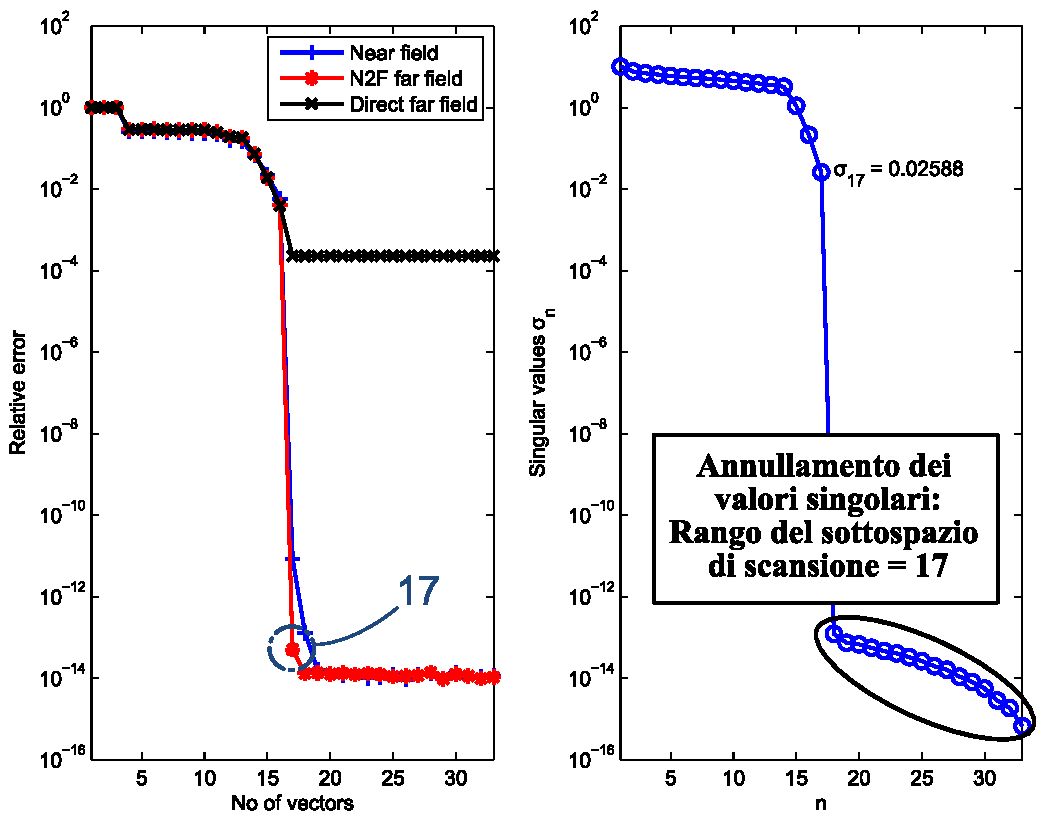
\includegraphics[width=7.5cm]{SVDerrorExp_33_0,75}}
%\only<2>{\vspace{-.904cm}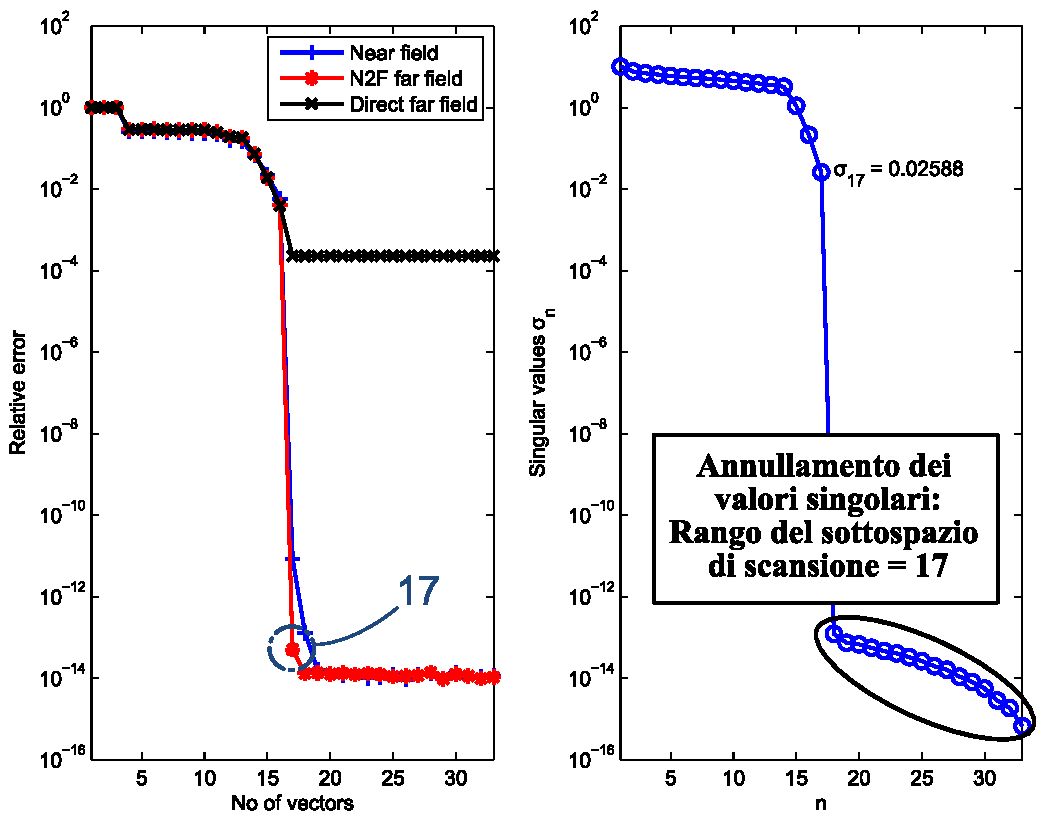
\includegraphics[width=5.5cm]{SVDerrorExp_33_0,75}}
%\end{center}
%\pause
%\begin{itemize}
%\only<2>{
%\begin{colorblock}{mycolor}{mycolor}{}
%\vspace{-.5cm}
%$\alpha$ in scansione lineare dipende dal \alert{numero di elementi radianti} (rango del sottospazio di scansione) e dalle loro \alert{distanze relative} \pause
%\end{colorblock}
%}
%}

%\frame{
%\frametitle{Analisi del campo vicino in \textbf{scansione planare} - campo scalare $\psi$}
%\begin{center}
%\vspace{-.2cm}
%Array planare di 3x5 sorgenti puntiformi equispaziate di $\nicefrac{\lambda}{2}$ \\[-.5cm]
%\end{center}
%\begin{itemize}
%\item $(\theta_{s_i},\phi_{s_i})$ da scansioni lineari lungo $x$ e $y$ \\[.4cm] 
%\begin{columns}[cc]
%\column{6cm}
%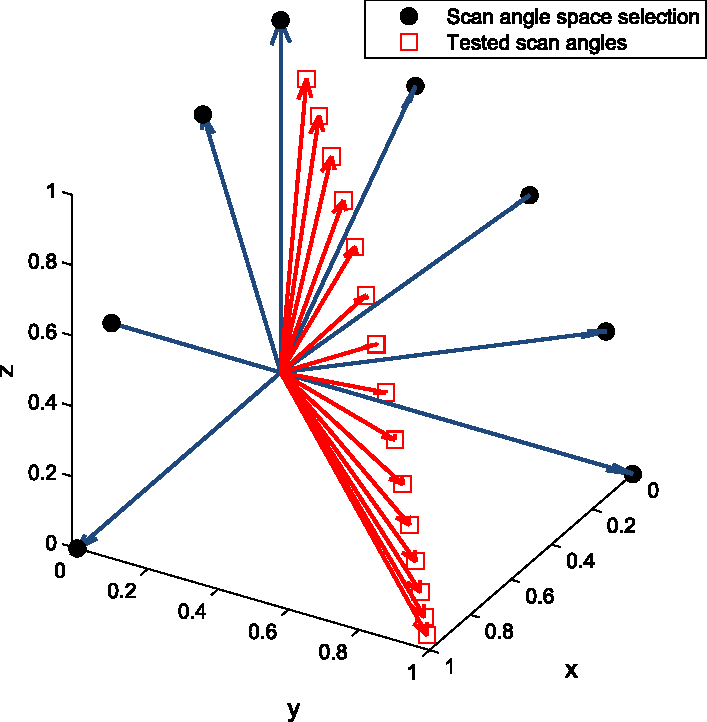
\includegraphics[width=5cm]{sel3x5angles}
%\column{4cm}
%$\color{red} \varepsilon_\mrm{trasformato} \color{black} \approx 0.5$
%\end{columns} 
%\end{itemize}
%}

%\frame{
%\frametitle{Analisi del campo vicino in \textbf{scansione planare} - campo scalare $\psi$}
%\begin{center}
%\vspace{-.2cm}
%\only<1>{\vspace{-.16cm}}
%\only<2>{\vspace{-.29cm}}
%\only<3>{\vspace{-.37cm}}
%Array planare di 3x5 sorgenti puntiformi equispaziate di $\nicefrac{\lambda}{2}$ \\[.4cm]
%\only<1>{\vspace{-.2cm}}
%\end{center}
%\begin{itemize}

%\begin{center}
%\only<1>{\begin{itemize}
%\item $(\theta_{s_i},\phi_{s_i})$ su traiettoria spirale elicoidale per l'emisfero nord \\[.1cm]
%\end{itemize}}
%\only<1>{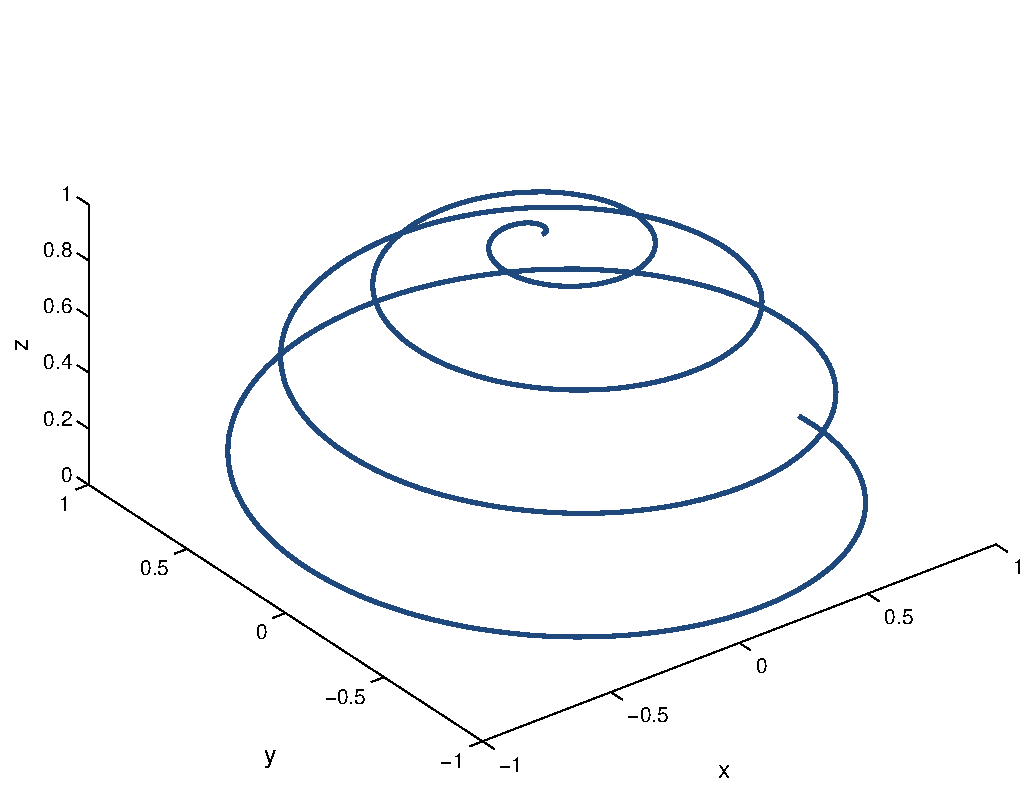
\includegraphics[width=6cm]{traj}}
%\only<2>{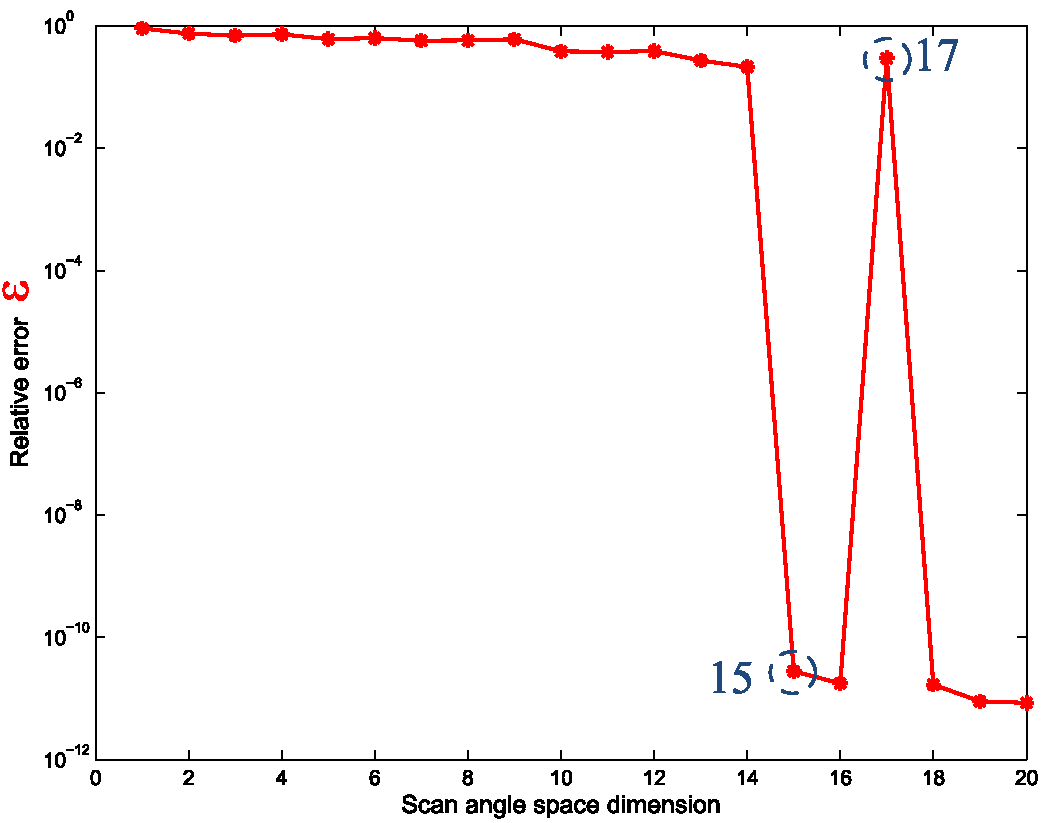
\includegraphics[width=7cm]{spirHelErrorSVD}}
%\only<3>{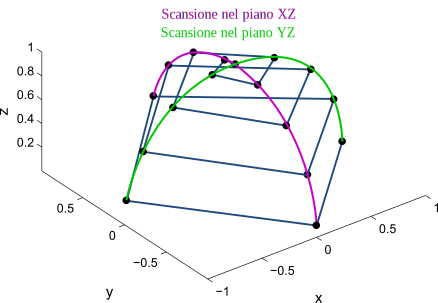
\includegraphics[width=7.75cm]{spirHeltraj17}}
%\end{center} 
%\end{itemize}

%}

%\frame{

%\begin{itemize}
%\item $\mat W$ costituisce uno \alert{spazio di \itt{test}} per la relazione Ingresso-Stato \\[.2cm] \pause
%\item Proiezione di Galerkin $\mat W = \mat V$ mantiene il \itt{matching} negli direzioni di scansione selezionati $(\theta_{s_i}, \phi_{s_i})$ %\pause
%\item Proiezione Petrov-Galerkin $\mat W :$ $$\mrm{span} \ \left \{ \bigcup_{i=1}^\alpha  \ \vect{z}_i(\theta_{i}, \phi_{i}) \right \} \subseteq \colspan{\mat W}$$ con $\vect{z}_i$ soluzioni del \alert{problema duale} $$\mat{A}^H \ \vect z(\theta, \phi) = \sum_{q=-Q}^Q \Omega_q(\theta) \mat{c}_q(\phi) $$ oltre al \itt{matching} negli direzioni di scansione (globale) assicura anche il \itt{matching} negli angoli di osservazione selezionati $(\theta_{i}, \phi_{i})$ (locale) $\Rightarrow$  \alert{Ulteriori $\alpha$ soluzioni da calcolare}
%\end{itemize}
%}
%\frame{
%\frametitle{Misura dell'errore indotto sul \itt{pattern}}
%\begin{itemize}
%\item 
%\item 
%\item 

%\end{itemize}
%}

\section{Esempio numerico e conclusioni}
\subsection{Array di 3x5 antenne a patch}

\frame
{
  \frametitle{Progetto di array planare di 3x5 antenne a patch con HFSS}
	\begin{center}
\only<1-2>{\vspace{-1cm}}
\only<2>{\vspace{-.235cm}}
\only<3>{\vspace{-1.235cm}}
		$f$ = 2.35 GHz, $\ \Delta x = \Delta y = \nicefrac{\lambda_0}{2}$ \\[.5cm]
\only<1>{\vspace{.2cm}}
		\only<1>{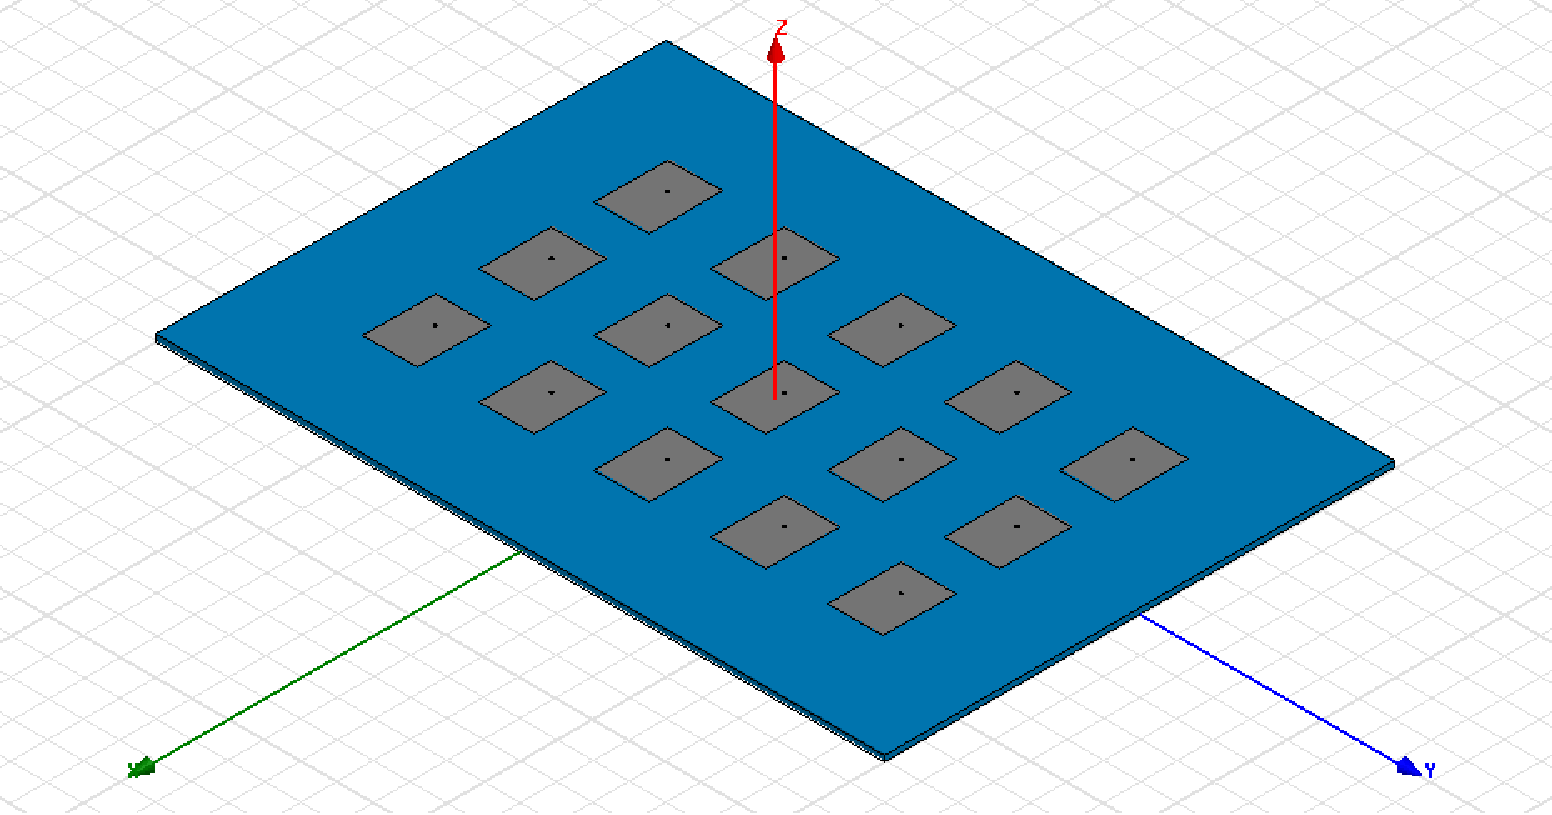
\includegraphics[width=8cm]{HFSS3x5array}}
		%\only<2>{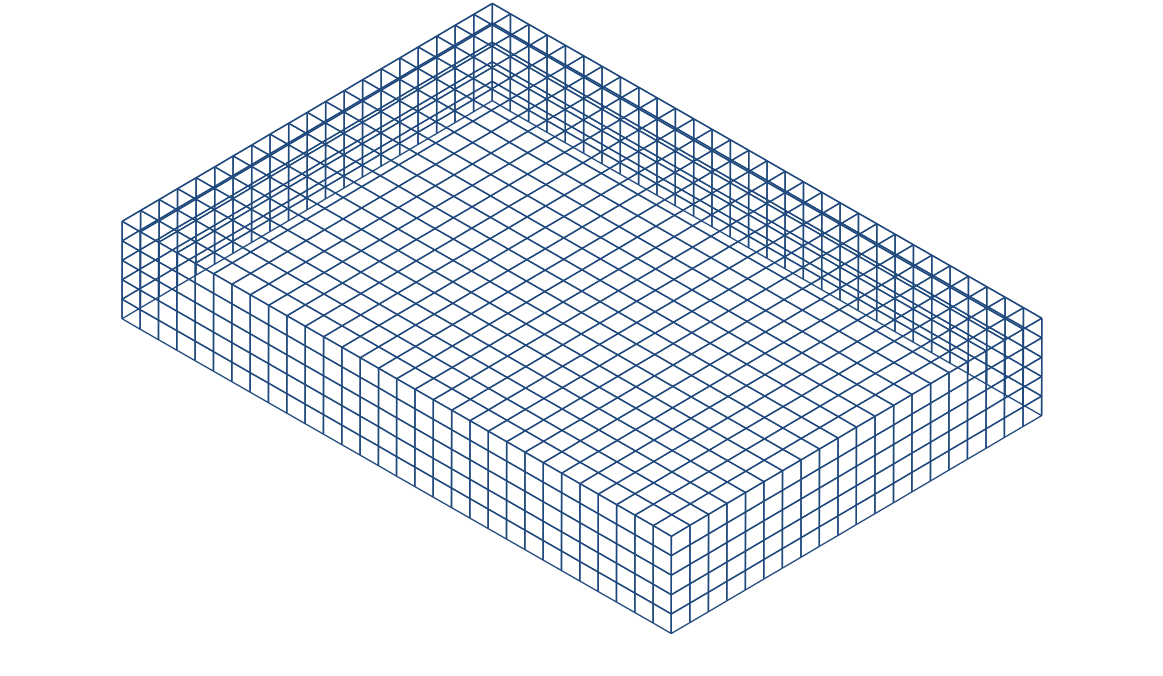
\includegraphics[width=8cm]{HFSS3x5arraySMPL}\\
%1100 campioni $\tilde{\mbfit E}, \tilde{\mbfit H}$ su $\mrm{\Gamma_R}$, risoluzione $\nicefrac{\lambda_0}{10}$
%}
		\only<2>{ 
\vspace{.4cm}
\begin{columns}[cc]
\column{7cm}
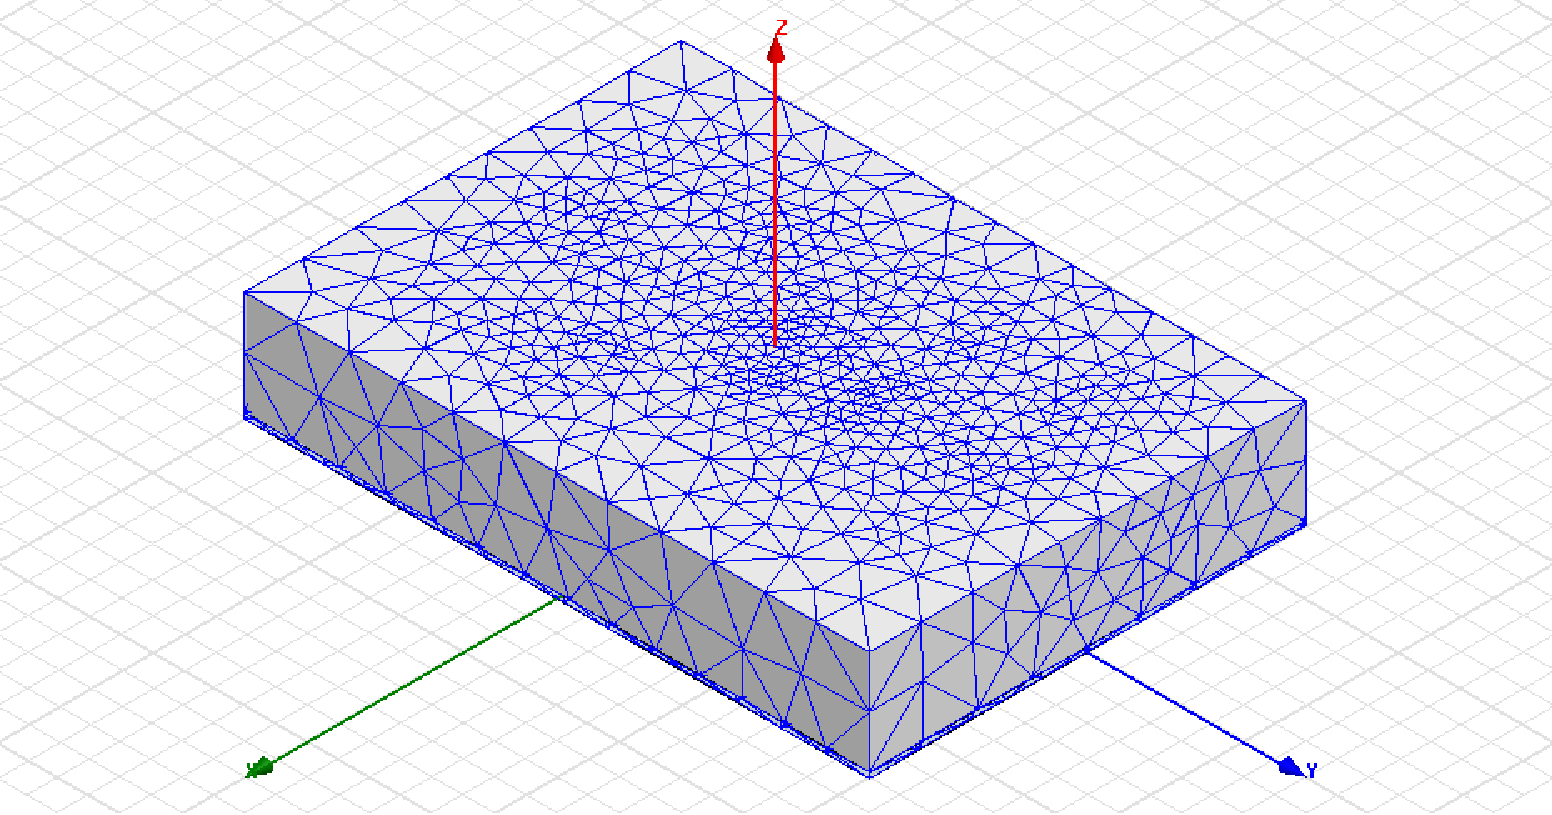
\includegraphics[width=7cm]{HFSS3x5MeshFull}
\column{5cm}
\begin{itemize}
\item Funzioni di base del $1^o$ ordine\\
\item \itt{Mesh} \itt{h-adaptive}  con tetraedri ($h_\mrm{max}=\nicefrac{\lambda}{3}$)
\end{itemize}
\end{columns}
}
		\only<3>{
\vspace{.4cm}
\begin{columns}[cc]
\column{7cm}

\includegraphics[width=7cm]{HFSS3x5Mesh}
\column{5cm}
\begin{itemize}
\item Funzioni di base del $1^o$ ordine\\
\item \itt{Mesh} \itt{h-adaptive} con tetraedri  ($h_\mrm{max}=\nicefrac{\lambda}{3}$)
\end{itemize}
\end{columns}
}
	\end{center}
}
\frame{
\only<1>{\frametitle{Pattern \itt{broadside} ($\theta_s$=0\�,$\phi_s$=0\�): HFSS}}
\only<2>{\frametitle{Pattern \itt{broadside} ($\theta_s$=0\�,$\phi_s$=0\�): Implementazione propria}}
\begin{center}
\only<1> {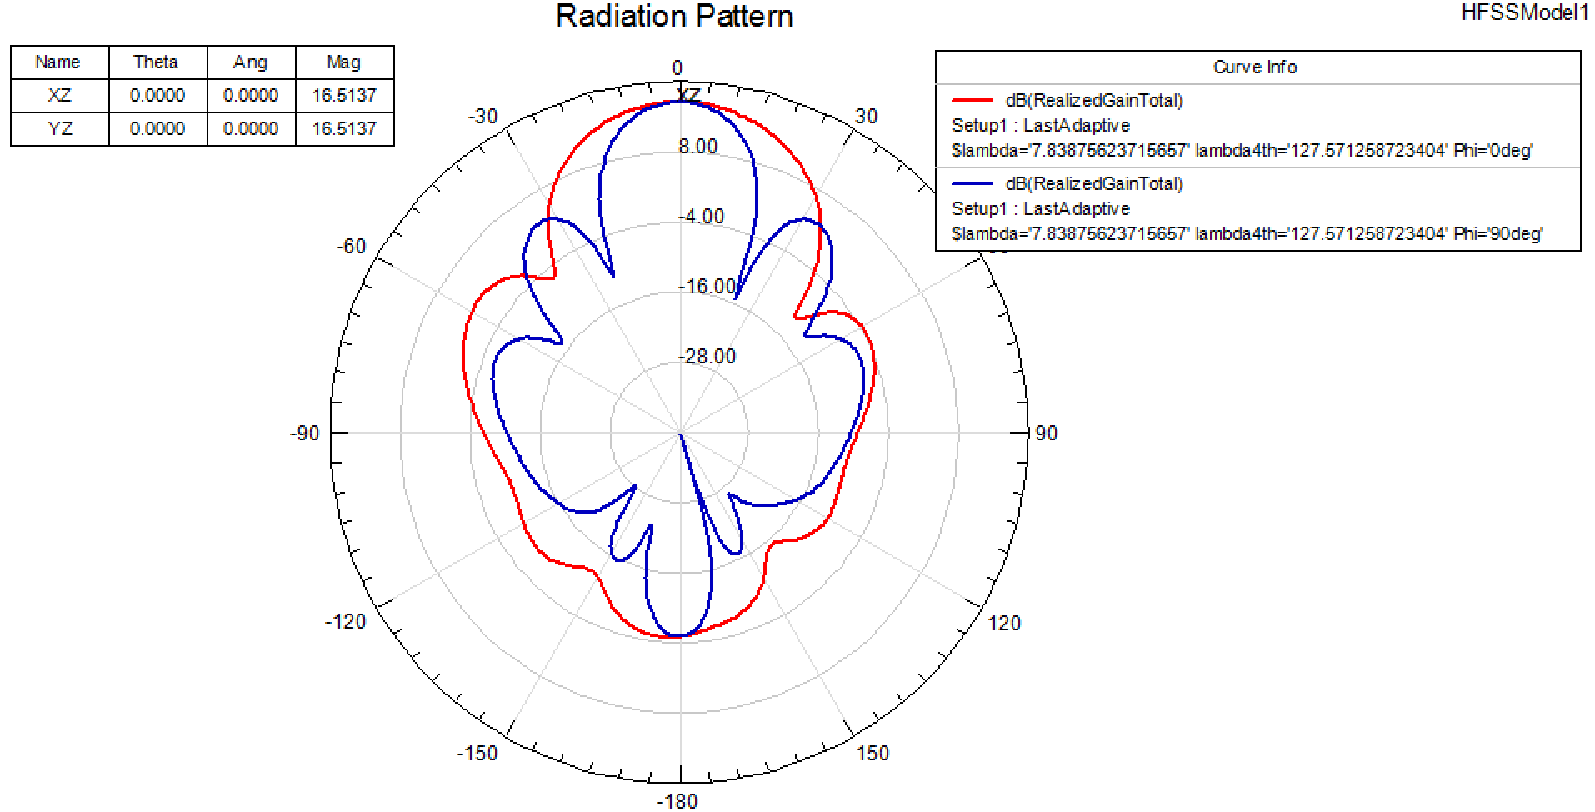
\includegraphics[width=8cm]{HFSS3x5pattern}\\
\footnotesize
\begin{itemize}
\item 358'\! 648 incognite
\item Memoria richiesta: \alert{$\approx$ 1.5 GB}
\item Tempo di computazione \alert{$\approx$ 38 min}
\item La computazione del \itt{pattern} sui piani a $\phi=0\�$ e $\phi=90\�$ richiede \alert{$\approx$ 35 s}
\end{itemize}
}
\only<2> {
\begin{columns}[cc]
\column{5cm}
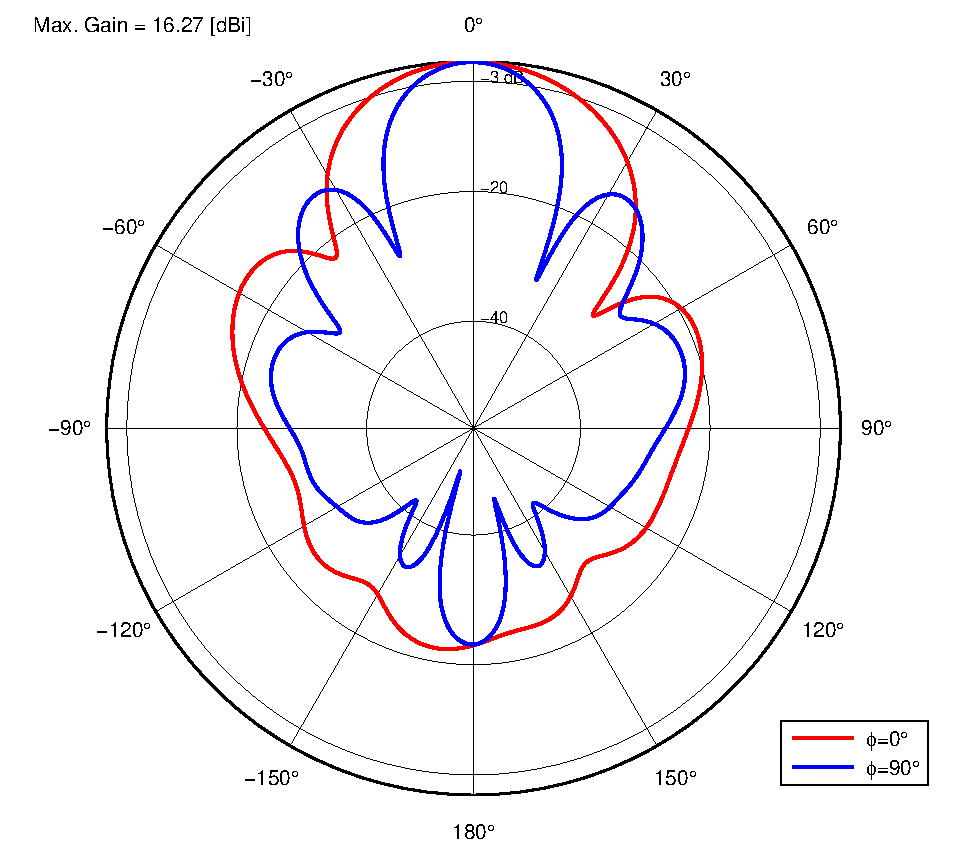
\includegraphics[width=5cm]{patchPatternBSnearABC} 
\column{7cm}
%\begin{center}
\footnotesize \itt{Mesh} e caratteristiche dei materiali estratti\\[-.1cm] dal progetto con HFSS \normalsize \\[.3cm]
%\end{center} 
\begin{itemize}
\item 358'\! 648 incognite
\item 1100 campioni $\tilde{\mbfit E}, \tilde{\mbfit H}$ su $\mrm{\Gamma_R}$, risoluzione $\nicefrac{\lambda_0}{10}$
\item 21 coefficienti di Fourier%($\color{red}\varepsilon_\mrm{trasformato} \color{black} \approx 10^{-4}$)
%(errore ininfluente sulla trasformazione da campi vicini a campi lontano)
\item 60 piani a $\phi$ costante per una risoluzione azimutale di $\Delta \phi = 3\�$
\end{itemize}
\end{columns}
\footnotesize
\begin{itemize}
\item Memoria richiesta dal modello di radiazione completo: \alert{$\approx$ 625 MB} 
\item Tempi di computazione: \Big \{ \begin{tabular*}{5cm}[h]{l}
Costruzione delle matrici: \alert{$\approx 20$ min}\\
Soluzione del sistema d'ingresso: \alert{$\approx 25$ min}
\end{tabular*}
\item Parametrizzazione $\Rightarrow$ la computazione del \itt{pattern} sui piani a $\phi=0\�$ e $\phi=90\�$ richiede \alert{150 ms} (fattore 233 rispetto a HFSS)
\end{itemize}
}
\end{center}
}
\frame
{
  \frametitle{Riduzione del modello per scansione nel piano XZ}
\begin{itemize}
\item $\alpha$ direzioni di scansione $(\theta_{s_i} \in \{ 0\�, 90\�, 45\�, 22.5\�, 67.5\�,\ldots \}, \phi_{s_i}=0\�)$
\end{itemize}
\begin{center}
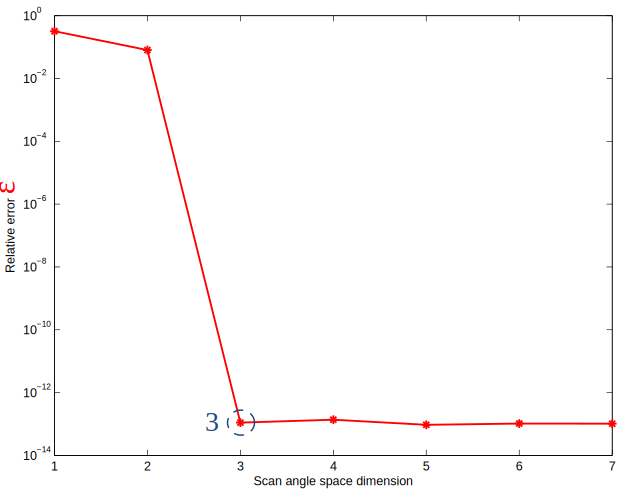
\includegraphics[width=7cm]{errorXZ}
\end{center}
}
\frame
{
  \frametitle{Riduzione del modello per scansione nel piano YZ}
\begin{itemize}
\item $\alpha$ direzioni di scansione $(\theta_{s_i} \in \{ 0\�, 90\�, 45\�, 22.5\�, 67.5\�,\ldots \}, \phi_{s_i}=90\�)$
\end{itemize}
\begin{center}
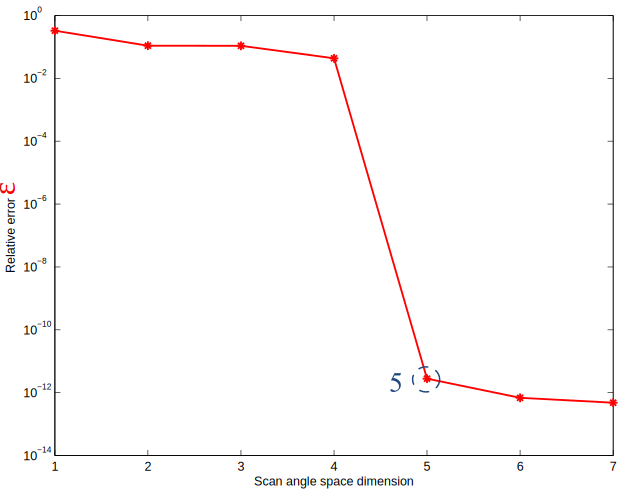
\includegraphics[width=7cm]{errorYZ}
\end{center}
}
\frame
{
  \frametitle{Riduzione del modello per scansione del semispazio superiore}
	%\begin{itemize}
%\item Proiezione Galerkin $\mat V = \mat W$ con $(\theta_{s_i},\phi_{s_i})$ su traiettoria spirale elicoidale per l'emisfero nord \\[.2cm] %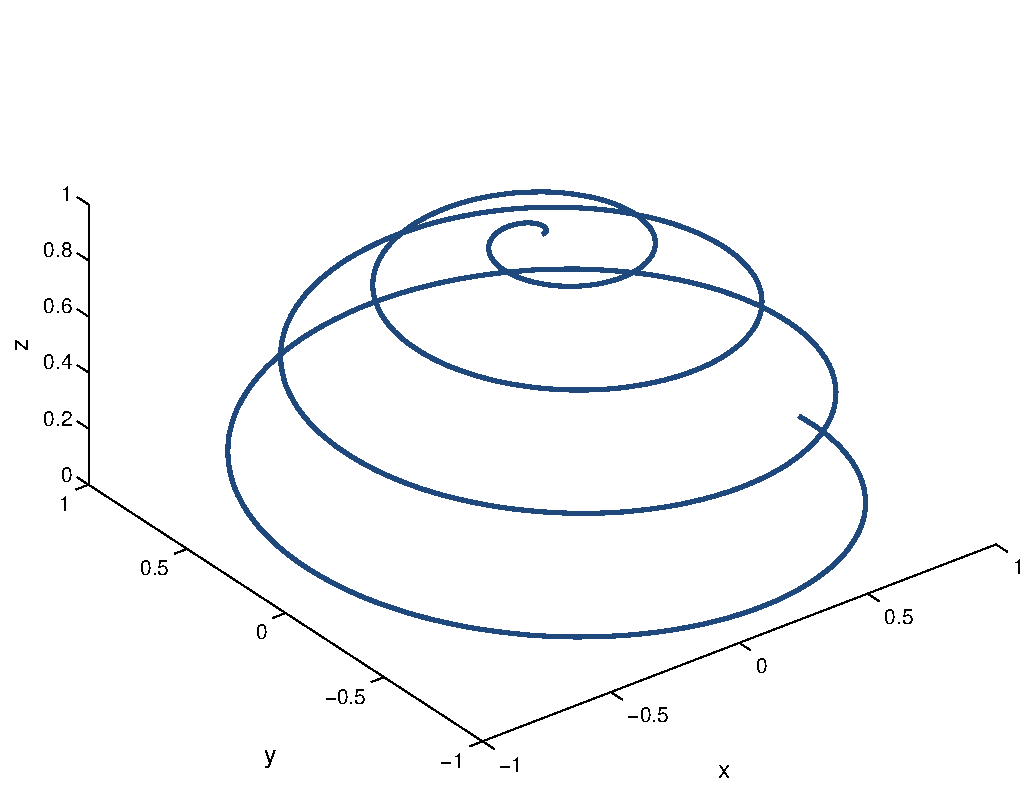
\includegraphics[width=5cm]{traj} 
%\pause
\begin{center}
\only<1>{\begin{itemize}
\item $\alpha$ direzioni di scansione $(\theta_{s_i},\phi_{s_i})$ individuate da punti equispaziati su di una traiettoria spirale elicoidale per l'emisfero nord\\[.1cm]
\end{itemize}}
\only<1>{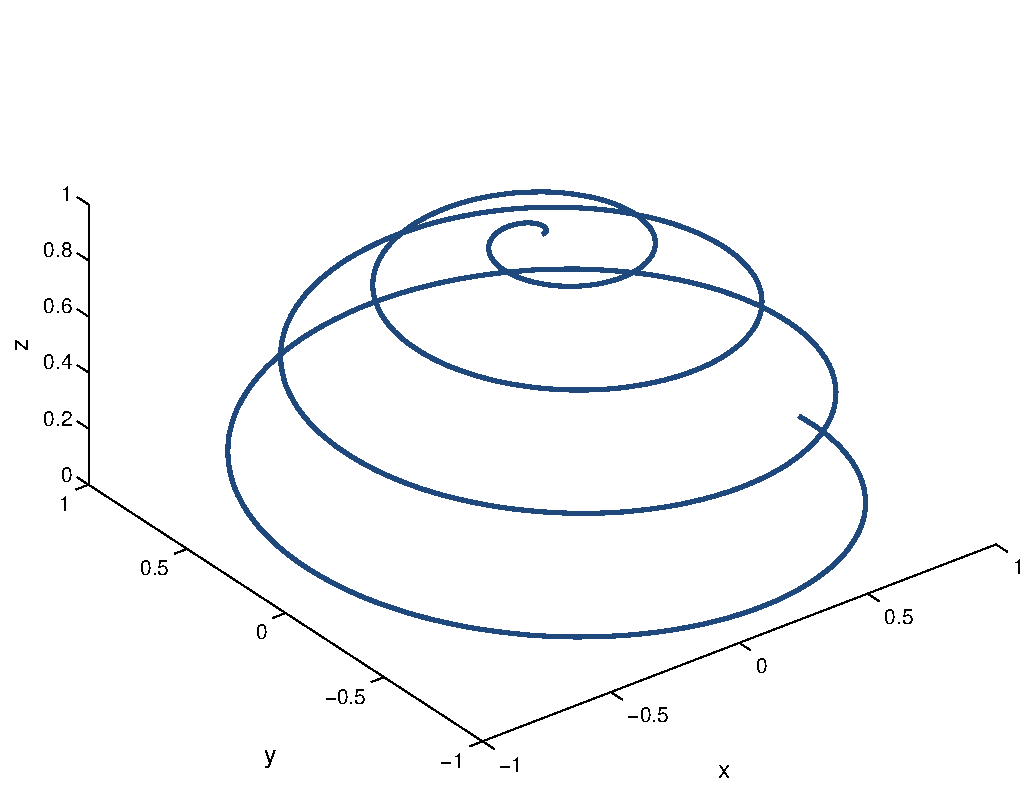
\includegraphics[width=6cm]{traj}}
\only<2>{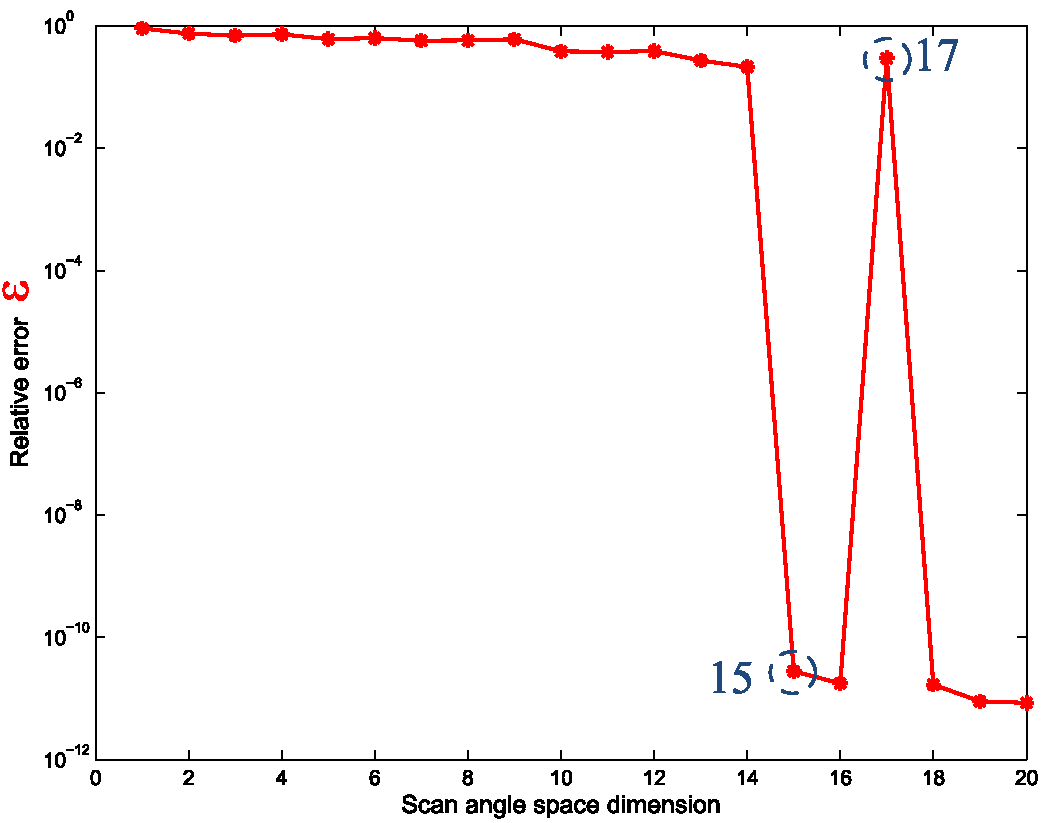
\includegraphics[width=7cm]{spirHelErrorSVD}}
\only<3>{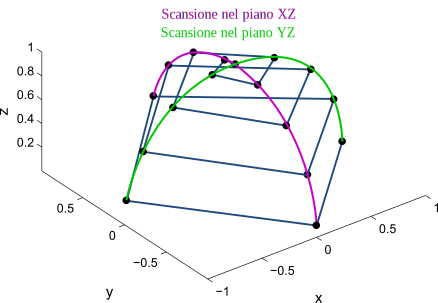
\includegraphics[width=7.75cm]{spirHeltraj17}}
\end{center}
}
\frame{
\frametitle{Riduzione del modello  per scansione del semispazio superiore}
\begin{itemize}
\item $\alpha$ = 15 (n$\mrm{^o}$ di elementi radianti)
\begin{itemize}
\item N$\mrm{^o}$ di incognite: \alert{358'\! 648 $\rightarrow$ 15} !!!
\item Memoria richiesta: \alert{625 MB $\rightarrow$ 1.5 MB} !!! 
\item Errore di riduzione della complessit\acgrave{a}: \alert{$\varepsilon \leq 10^{-11}$} !!!
\end{itemize}
\end{itemize}
}

\frame
{
\vspace{-.1cm}
\begin{center}
\movie[width=8cm,height=6cm, poster]{}{MovScan.avi} \\
\footnotesize 
$\Delta \theta = 0.12 \�, \Delta \phi = 3 \� $
\end{center}
%\pause
\vspace{-.1cm}
%\begin{center}
\begin{columns}
\scriptsize \hspace{.5cm}
\column{7cm}
Tempo di \itt{frame} per la risoluzione scelta: \\[-.1cm]
\begin{itemize} 
\item per \alert{HFSS}: \alert{7 min 10 s}
\item \vspace{-.1cm} per il modello \alert{completo} parametrizzato: \alert{520 ms}
\item \vspace{-.1cm} per il modello \alert{ridotto} parametrizzato: \alert{63 ms}
\end{itemize}
\column{.5cm}
\vspace{-.8cm} $\Rightarrow$ \hspace{.5cm}
\column{4cm}
Elaborazione filmato: \\[-.1cm]
\begin{itemize}
\item \alert{10 ore 20 min}
\item \vspace{-.1cm} \alert{$\approx$ 1 min 3 s}
\item \vspace{-.1cm} \alert{$\approx$ 8 s}
\end{itemize}
\end{columns}
%\end{center}
}

%\subsection{40 antenne Vivaldi in doppia polarizzazione}
%\frame{
%\frametitle{}
\subsection{Conclusioni}

\frame{

\frametitle{Conclusioni}
\begin{itemize}
\item Tecnica promettente per l'analisi di array fasati di grandi dimensioni %\pause
\item Possibilit\acgrave{a} di parametrizzare il modello in frequenza ($k_0$) e nelle caratteristiche dei materiali ($\dyad{\epsilon}_r, \ \dyad{\mu}_r, \ \dyad{\sigma} $) $\Rightarrow$ Banda di lavoro e tolleranze di fabbricazione%\pause
\item Ottimizzazione su \itt{pattern} accurati
\end{itemize}

}

\frame{
\Large
\begin{center}
Vi ringrazio per l'attenzione
\end{center}
}


%}


\end{document}
